\documentclass[sigconf]{acmart}

\newcommand\hmmax{0}
\newcommand\bmmax{0}

\usepackage[percent]{overpic}
\usepackage{algorithm}
\usepackage{algorithmic}

\renewcommand{\algorithmicrequire}{\textbf{Input:}}
\renewcommand{\algorithmicensure}{\textbf{Output:}}

%\usepackage{multicol,amsmath,amsthm}

%\usepackage[T1]{fontenc}
%\usepackage{lmodern}

\usepackage{amsmath}
\usepackage{amsfonts}
\usepackage{amsthm}
\usepackage{amssymb}

\usepackage{graphicx}
\usepackage[export]{adjustbox}
\usepackage{url}
\usepackage{xspace}

%\usepackage{fancyvrb}
%\usepackage{bm}

\usepackage[format=plain,labelfont=up]{caption}
\usepackage{multirow}
\usepackage{xcolor}
\usepackage{colortbl}
\usepackage{afterpage}
\usepackage{booktabs}
\usepackage{comment}

%\usepackage[dvipsnames,table]{xcolor}
\usepackage{pgf}
\usepackage{pgfplots,pgfplotstable}
\usepackage{tikz}
\usepackage{tikzscale}
\usetikzlibrary{shapes,backgrounds}
\usetikzlibrary{arrows,shapes,fit,automata,positioning,decorations,calc}
\usetikzlibrary{spy,backgrounds}
\usetikzlibrary{arrows.meta}
\usepackage{siunitx}
\pgfplotsset{compat=1.12}


\usepackage{pslatex} % -- times instead of computer modern, especially for the plain article class
%\usepackage[colorlinks=false,bookmarks=false]{hyperref}
\usepackage{booktabs}

\usepackage{multirow}
%\usepackage{cite}
\usepackage[normalem]{ulem} %for striking out text
%

\usepackage{calligra} %
\usepackage{mathtools}


\usepackage{dblfloatfix} %allows floats to be at bottom of page

%tikz and associated stuff
%\usepackage{verbatim}
\usetikzlibrary{shapes,backgrounds}
\usetikzlibrary{arrows,fit,automata,positioning,decorations,calc}
\usetikzlibrary{spy}
\usetikzlibrary{matrix,chains,decorations.pathreplacing}
%\usetikzlibrary{arrows.meta}

\usepackage{caption}
\usepackage{subcaption}

\usetikzlibrary{patterns}

\usepackage[english]{babel}
\usepackage{blindtext}

\usepackage{acronym}

%\usepackage[subtle]{savetrees}

%\usepackage{flushend} % even out the last page, but use only at the end when there is a bibliography

\newcommand\defeq{\stackrel{\mathclap{\scriptsize\mbox{def}}}{=}}
\newcommand{\code}[1]{{\small{\texttt{#1}}}}

% fatter TT font
\renewcommand*\ttdefault{txtt}
% another TT, suggested by Alex
% \usepackage{inconsolata}
% \usepackage[T1]{fontenc} % needed as well?

\usepackage{float}
\newcommand{\todo}[1]{{\color{orange}(TODO: #1)}}
\newcommand{\hammond}[1]{{\color{blue} Hammond: #1}}
\newcommand{\matthew}[1]{{\color{red} Matthew: #1}}
\newcommand{\changed}[1]{{\color{red}#1}}

\theoremstyle{definition}
\newtheorem{definition}{Definition}[section] % definition numbers are dependent on theorem numbers
\theoremstyle{example}
\newtheorem{example}[definition]{Example} % same for example numbers
\theoremstyle{theorem}
\newtheorem{thm}[definition]{Theorem}
\newtheorem{lemma}[definition]{Lemma}
%\newtheorem{defn}{definition}[section]
%\newtheorem{exmp}{example}[section]
%\newtheorem{rem}{remark}

\pgfplotsset{compat=1.11,
	/pgfplots/ybar legend/.style={
		/pgfplots/legend image code/.code={
			\draw[##1,/tikz/.cd,bar width=3pt,yshift=-0.2em,bar shift=0pt]
			plot coordinates {(0cm,0.8em)};
		},
	},
}

\newcounter{remarks}
\newtheorem{remark}{Remark}

\include{preamble-listingsconf}
\newcommand{\efalgo}{\ensuremath{{E_{\varphi}^*}}}
\DeclareSymbolFont{bbold}{U}{bbold}{m}{n}
\DeclareSymbolFontAlphabet{\mathbbold}{bbold}
\newcommand{\df}{\stackrel{df}{=}}
\newcommand{\dfs}{=_{\scriptstyle{df}}}
\newcommand{\miff}{\mbox{\it iff\/}}
\newcommand{\mi}[1]{\ensuremath{\mathit{#1}}\xspace}
\newcommand{\ignore}[1]{{}}
\newcommand{\Scott}{\ensuremath{\mathbb S}\xspace}
\newcommand{\Real}{\ensuremath{\mathbb R}\xspace}
\newcommand{\Bool}{\ensuremath{\mathbb B}\xspace}
\newcommand{\Nat}{\ensuremath{{\mathbb N}}\xspace}
\newcommand{\cNat}{\ensuremath{{\mathbb N}_{\infty}}\xspace}
\newcommand{\modd}{\ensuremath{\mathrel{\textit{mod}}}\xspace}
\newcommand{\maxd}{\ensuremath{\textit{max}}\xspace}
\newcommand{\mind}{\ensuremath{\textit{min}}\xspace}
\newcommand{\zero}{\ensuremath{\mathbb{0}}\xspace}
\newcommand{\one}{\ensuremath{\mathbb{1}}\xspace}

\newcommand{\pr}[1]{{\textsf{\color{red} \small{[#1 -pr-]}}}}
\newcommand{\hp}[1]{{\textsf{\color{red} \small{[#1 -hp-]}}}}
\newcommand{\hw}[1]{{\textsf{\color{red} \small{[#1 -km-]}}}}
\newtheorem{prop}{Proposition}

\newcommand{\bbb}{\mathbb{B}}
\newcommand{\bbn}{\mathbb{N}}
\newcommand{\bbr}{\mathbb{R}}
\newcommand{\Rnn}{{\bbr}_{\geq 0}}
\newcommand{\calL}{{\mathcal L}}
\newcommand{\calP}{{\mathcal P}}
\newcommand{\calA}{{\mathcal A}}
\newcommand{\calD}{{\mathcal D}}
\newcommand{\calV}{{\mathcal V}}
\newcommand{\exec}{\mathit{exec}}
\newcommand{\true}{\ensuremath{\mathsf{true}}}
\newcommand{\false}{\ensuremath{\mathsf{false}}}
\newcommand{\pref}{\preccurlyeq}
\newcommand{\sem}[1]{[\!\left[#1\right]\!]}
\newcommand{\bin}[1]{\overrightarrow{#1}}

\newcommand{\ef}{\ensuremath{E_{\varphi}}}

\newcommand{\red}[1]{{\color{red}#1}}

\DeclareMathOperator{\Run}{Run}

\newcommand{\ptick}{\mathsf{ptick}}
\newcommand{\editI}{\mathsf{editI_{\varphi_I}}}
\newcommand{\editO}{\mathsf{editO_{\varphi}}}
\newcommand{\editIaut}{\mathsf{editI_{\calA_{\varphi_I}}}}
\newcommand{\editOaut}{\mathsf{editO_{\calA_\varphi}}}
\newcommand{\randEditI}{\mathsf{{rand}\mbox{-} editI_{\varphi_{I}}}}
\newcommand{\randEditO}{\mathsf{{rand}\mbox{-} editO_{\varphi}}}
\newcommand{\randEditIaut}{\mathsf{{rand}\mbox{-} editI_{\calA_{\varphi_{I}}}}}
\newcommand{\randEditOaut}{\mathsf{{rand}\mbox{-} editO_{\calA_\varphi}}}

\newcommand{\selEditI}{\mathsf{{sel}\mbox{-} editI_{\varphi_{I}}}}
\newcommand{\selEditO}{\mathsf{{sel}\mbox{-} editO_{\varphi}}}
\newcommand{\selEditIaut}{\mathsf{{sel}\mbox{-} editI_{\calA_{\varphi_{I}}}}}
\newcommand{\selEditOaut}{\mathsf{{sel}\mbox{-} editO_{\calA_\varphi}}}

\newcommand{\dist}{\mathsf{dist}}

\newcommand{\minEditI}{\mathsf{{minD}\mbox{-} editI_{\varphi_{I}}}}
\newcommand{\minEditO}{\mathsf{{minD}\mbox{-} editO_{\varphi}}}
\newcommand{\minEditIaut}{\mathsf{{minD}\mbox{-} editI_{\calA_{\varphi_{I}}}}}
\newcommand{\minEditOaut}{\mathsf{{minD}\mbox{-} editO_{\calA_\varphi}}}

\newcommand{\readInp}{\mathsf{read\_in\_chan}}
\newcommand{\readOut}{\mathsf{read\_out\_chan}}
\newcommand{\release}{\mathsf{release}}
%\texttt{ptick}

\newcommand{\okI}{\mathit{OK\_solutions_I}}
\newcommand{\okO}{\mathit{OK\_solutions_O}}
%%%%%%%%%%%%%%%%%%%%%%%%%%%%%%%


\newcommand{\squishlist}{
	\begin{list}{$\bullet$}
		{ \setlength{\itemsep}{0pt}
			\setlength{\parsep}{1pt}
			\setlength{\topsep}{1pt}
			\setlength{\partopsep}{0pt}
			\setlength{\leftmargin}{0.9em}
			\setlength{\labelwidth}{1.5em}
			\setlength{\labelsep}{0.4em} } }
	\newcommand{\squishend}{
\end{list}  } 

%\DeclareRobustCommand*\cal{\@fontswitch\relax\mathcal}

\newenvironment{abbreviations}{
	\@restonecolfalse
	\chapter*{List of \abbreviationsname}
	\@mkboth{\abbreviationsname}
	{\abbreviationsname}
}
{\newpage\@mkboth{}{}}
\newcommand\abbreviationsname{Abbreviations}


\begin{filecontents*}{avdta.tikz}
	

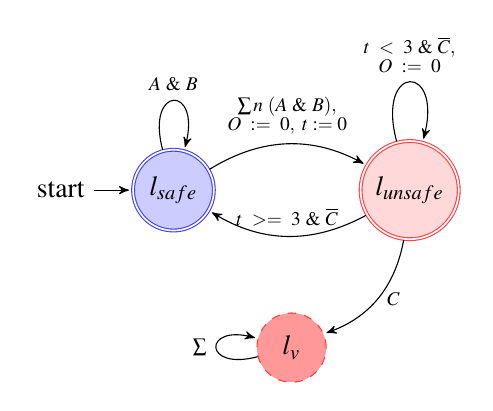
\begin{tikzpicture}[>=stealth',shorten >=1pt,auto,node distance=3cm, scale = 1, transform shape]

\tikzstyle{accept} = [draw=blue!75,fill=blue!20]
\tikzstyle{violate} = [draw=red!75,fill=red!40, dashed]
\tikzstyle{unstable} = [draw=red!75,fill=red!15]

\node[state, initial, accepting, accept] (A) {$l_{safe}$};
\node[state, accepting, accept, unstable] (B) [right of=A] {$l_{unsafe}$};
\node[state, violate]         (C) [below of=B, yshift=1cm, xshift=-1.5cm]  {$l_v$};

\path[->] 
		(A) edge [loop above]       node [above]  
		{
			\scriptsize$\let\scriptstyle\textstyle\substack{A~\&~B}$
		} (A)
		
		(A) edge [bend left]		node [above]  
		{
			\scriptsize$\let\scriptstyle\textstyle\substack{\sum\textbackslash~(A~\&~B),\\O~:=~0,~t := 0}$
		} (B)
	
		(B) edge [loop above]		node [above]  
		{
			\scriptsize$\let\scriptstyle\textstyle\substack{t~<~3~\&~\overline{C},\\O~:=~0}$
		} (B)
	
		(B) edge [bend left]				node [above]  
		{
			\scriptsize$\let\scriptstyle\textstyle\substack{t~>=~3~\&~\overline{C}}$
		} (A)
		
		(B) edge [bend left]			node [right]  
		{
			\scriptsize$\let\scriptstyle\textstyle\substack{C}$
		} (C)
	
		(C) edge [loop left]		node [left]  
		{
			\scriptsize$\let\scriptstyle\textstyle\substack{\sum}$
		} (C)
		;

\end{tikzpicture}
\end{filecontents*}
\begin{filecontents*}{avgraph.tikz}
	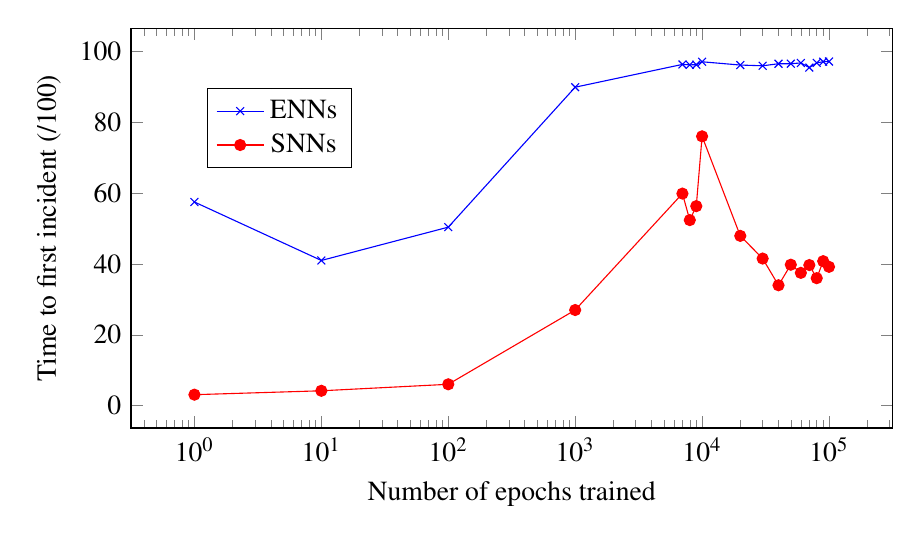
\begin{tikzpicture}
\begin{semilogxaxis}[
xlabel={Number of epochs trained},
ylabel={Time to first incident (/100)},
x=0.7cm,
y=0.45mm, 
legend style={at={(0.1,0.75)},anchor=west}]

\addplot[color=blue,mark=x] coordinates {
	(0, 52.5)
	(1, 57.5)
	(10, 41.0)
	(100, 50.4)
	(1000, 89.9)
	(7000, 96.33)
	(8000, 96.21)
	(9000, 96.24)
	(10000, 97.07)
	(20000, 96.15)
	(30000, 95.94)
	(40000, 96.52)
	(50000, 96.53)
	(60000, 96.74)
	(70000, 95.44)
	(80000, 96.75)
	(90000, 97.09)
	(100000, 97.14)
};


\addplot[color=red,mark=*] coordinates {
	(0, 2.95)
	(1, 3.12)
	(10, 4.22)
	(100, 6.05)
	(1000, 27.01)
	(7000, 59.87)
	(8000, 52.39)
	(9000, 56.33)
	(10000, 76.03)
	(20000, 47.94)
	(30000, 41.54)
	(40000, 34)
	(50000, 39.8)
	(60000, 37.5)
	(70000, 39.7)
	(80000, 36)
	(90000, 40.8)
	(100000, 39.2)
};


\legend{ENNs, SNNs}
\end{semilogxaxis}%
\end{tikzpicture}%
\end{filecontents*}
\begin{filecontents*}{avgraphacc.tikz}
	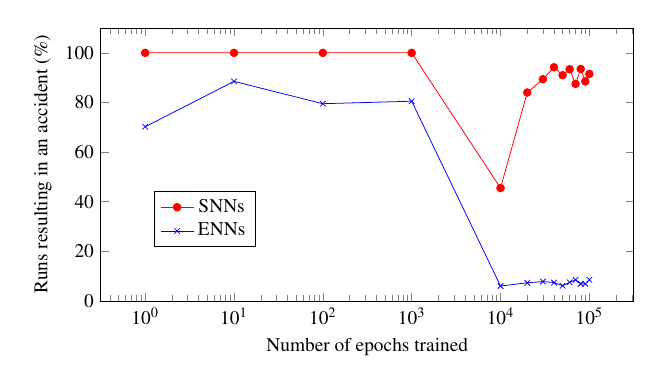
\begin{tikzpicture}[scale=0.7]
\begin{semilogxaxis}[
xlabel={Number of epochs trained},
ylabel={Runs resulting in an accident (\%)},
x=0.7cm,
y=0.45mm, 
ymin=0,
legend style={at={(0.1,0.3)},anchor=west}]

\addplot[color=red,mark=*] coordinates {
	(0, 100)
	(1, 100)
	(10, 100)
	(100, 100)
	(1000, 100)
	(10000, 45.5)
	(20000, 84.0)
	(30000, 89.4)
	(40000, 94.2)
	(50000, 91.0)
	(60000, 93.4)
	(70000, 87.5)
	(80000, 93.5)
	(90000, 88.5)
	(100000, 91.5)
};

\addplot[color=blue,mark=x] coordinates {
	(0, 75.7)
	(1, 70.2)
	(10, 88.5)
	(100, 79.5)
	(1000, 80.5)
	(10000, 6.0)  
	(20000, 7.3)
	(30000, 7.8)
	(40000, 7.4)
	(50000, 6.1)
	(60000, 7.5)
	(70000, 8.5)
	(80000, 6.9)
	(90000, 6.9) 
	(100000, 8.5) 
};

\legend{SNNs, ENNs}
\end{semilogxaxis}%
\end{tikzpicture}%
\end{filecontents*}
\begin{filecontents*}{avpedrtesmall.tikz}
	\input{Content/fig/av-ped-rte-small.tex}
\end{filecontents*}

\copyrightyear{2019}
\acmYear{2019}
\setcopyright{acmlicensed}
\acmConference[]{ACM CASES}{October 2019}{New York, NY, USA}
%\acmPrice{15.00}
%\acmDOI{10.1145/1122445.1122456}
%\acmISBN{978-1-4503-9999-9/18/06}

\begin{document}

\title{Enhancing the safety of neural networks using runtime enforcement}

\ignore{
\author{Keyan Monadjem}
\affiliation{%
	\institution{University of Auckland}
	\city{Auckland, New Zealand} 
}
\email{kmon173@aucklanduni.ac.nz}

\author{Hammond Pearce}
\affiliation{%
	\institution{University of Auckland}
	\city{Auckland, New Zealand} 
}
\email{hammond.pearce@auckland.ac.nz}

\author{Srinivas Pinisetty}
\affiliation{%
	\institution{ Indian Institute of Technology Bhubaneswar}
	\city{Bhubaneswar, India} 
}
\email{spinisetty@iitbbs.ac.in}

\author{Partha S. Roop}
\affiliation{%
	\institution{University of Auckland}
	\city{Auckland, New Zealand} 
}
\email{p.roop@auckland.ac.nz}
}
\begin{abstract}
Neural networks are increasingly used in Cyber-Physical Systems (CPS),
where safety is paramount. Considering this, there are many recent
efforts on combining formal methods with neural networks. However,
none of the developed formal techniques are capable of verifying
timing requirements, which is essential for safe operation of CPS.

In this paper we make two novel contributions towards the design of a
new class of neural networks for safety called \acp{ENN}. First,
we provide a synchronous execution semantics of neural networks and
extend them with an unique run-time enforcement
framework to facilitate the mitigation of safety issues at
run-time. Second, we propose an enforcement algorithm that can
enforce policies that constrain neural networks by ensuring that all valued input and output remain policy
compliant and the response time of the network also remains policy
compliant. Thus, \acp{ENN} provide the first formal framework for
creating real-time systems based on neural networks.
Through two complex examples of safety-critical applications, we
demonstrate that the developed approach enhances the safety and quality
of the benchmarks. This paper paves the way towards the design of safer
neural networks using run-time enforcement.
\end{abstract}

\maketitle

\acrodef{WCRT}{Worst Case Reaction Time}
\acrodef{WCET}{Worst Case Execution Time}
\acrodef{SOT}{Start Of Tick}
\acrodef{EOT}{End Of Tick}
\acrodef{CPS}{Cyber-Physical Systems}
\acrodef{AI}{Artificial Intelligence}

\acrodef{ESS}{Energy Storage System}
\acrodef{SoC}{State of Charge}
\acrodef{MBD}{Model-Based Design}
\acrodef{FPGA}{Field-Programmable Gate Array}

\acrodef{CFG}{Control Flow Graph}
\acrodef{TCFG}{Timed Control Flow Graph}
\acrodef{TCCFG}{Timed Concurrent Control Flow Graph}
\acrodef{TCA}{Tick Cost Automata}

\acrodef{SA}{Security Automata}
\acrodef{SMT}{Satisfiability Modulo Theory}

\acrodef{EV}{Electric Vehicle}
\acrodef{ESS}{Energy Storage System}

\acrodef{ReLU}{Recitifed Linear Units}

\acrodef{ML}{Machine Learning}
\acrodef{NN}{Neural Network}
\acrodef{DNN}{Deep Neural Network}
\acrodef{SNN}{Synchronous Neural Network}
\acrodef{CNN}{Convolutional Neural Network}
\acrodef{SANN}{Synchronous Artificial Neural Network}
\acrodef{SCNN}{Synchronous Convolutional Neural Network}
\acrodef{SNN}{Synchronous Neural Network}
\acrodef{SSNN}{Safe Synchronous Neural Network}
\acrodef{ENN}{Enforced Neural Network}
\acrodef{ANN}{Artificial Neural Network}
\acrodef{RNN}{Recurrent Neural Network}
\acrodef{MLP}{Multi-layer Perceptron}
\acrodef{MNN}{Meta Neural Network}
\acrodef{MNN2C}{Meta Neural Network to C}

\acrodef{AV}{Autonomous Vehicle}
\acrodef{LiDAR}{Light Detection and Ranging}

\acrodef{VOC}{Visual Object Classes}
\acrodef{GTSRB}{German Traffic Sign Recognition Benchmark}

\acrodef{VDTA}{Valued Discrete Timed Automata}
\acrodef{DTA}{Discrete Timed Automata}
\acrodef{RE}{Run-time Enforcement}
\acrodef{RA}{Run-time Assurance}
\acrodef{RV}{Run-time Verification}
\acrodef{SA}{Security Automata}
\acrodef{OS}{Operating System}

\acrodef{OH}{Overhead}

\section{Introduction}
\acfp{ANN} have excelled in many applications such as
image and video processing to pattern classification. With the advent
of deep neural networks, they have excelled at achieving a level of
precision that far exceed humans, particularly those related to machine
vision.  More recently, their usage has moved from routine decision
making to more complex tasks that involve interaction with
automated control algorithms. This is especially concerning as deep neural networks are
being used in \acf{CPS} such as autonomous vehicles,
where no errors in control decisions may be tolerable. 

Any \ac{CPS}
consists of one or more distributed embedded systems, called the controllers, which are used
for controlling physical processes, called the plant.
In contract to the
\emph{data-driven} approach of neural networks, \ac{CPS} are often designed starting
from formal models~\cite{formal-methods}. These can be analysed at a
higher-level of abstraction prior to exposing the validated models to
automated code generation. Such approaches for
\ac{CPS} are classified as \emph{model-based design}. There are tools
such as SCADE~\cite{SCADE} based on this philosophy, which generate
correct-by-construction code compliant with safety standards.

While \ac{CPS} typically used conventional controllers designed using
mode-based approaches, recent applications such as
autonomous vehicles need data-driven processing using video-streams
from its sensors to automatically detect obstacles or traffic
signs. Such tasks are accomplished using \acfp{CNN}. These data-driven processing tasks need to interact with
conventional control tasks such as ABS-braking or adaptive cruise control.
Considering this, there is recent
research momentum in achieving convergence between the usual
model-driven approaches used in CPS and the more recent data-driven
approaches used in conventional AI based on statistical techniques~\cite{tripakis2018data}.

In~\cite{seshia2016towards} Seshia et al. consider some key challenges of 
using formal methods to verify neural networks. These include the
difficulty in creating mathematical models and the difficulty in
formalising requirements. There is also the
added challenge of designing scalable verification algorithms for
static analysis of neural networks. More recently, there has been
an attempt at developing abstract interpretation-based
solution~\cite{Gehr2018AI2SA} for the verification of CNNs. 
%They
%demonstrate through a series of reasonable benchmarks that their
%approach is both robust and scalable. 

\ignore{However, they mainly
concentrated on the issue of adversarial perturbations, which
significantly impact the robustness of CNNs. Also, we believe that the
scalability results over larger benchmarks of this approach need to be
considered. Finally, no existing work deals with the verification of
timing properties, which is an essential aspect of all CPS.}

CPS applications such as autonomous vehicles need real-time decision
making. This not only requires functional but also timing
validation. {\bf To the best of our knowledge,
there are no known methods for the systematic design of 
AI applications with timing requirements. This is our focus}.

We adopt a recent extension of of neural networks,
which are made periodic, termed \acfp{SNN}~\cite{sann}. 
This defines execution loops for \acp{ANN}, 
where in each loop, the network first reads
inputs from sensors, then processes the input in
a series of one or more logical ticks (a concept borrowed from synchronous programming languages~\cite{SynchronousLanguages12YearsLater}),
and finally it releases computed outputs.
This loop can be executed indefinitely.
Thanks to their underlying synchronous semantics, the loop timing properties can be computed, i.e. the loops are amenable to worst case execution time analysis~\cite{TheWCETProblem}. 
\acp{SNN} thus formalise the design of reactive controllers using neural networks.

We propose a new class of policies for enforcing safe behaviour
of \acp{SNN} using \ac{VDTA}. A \ac{VDTA} can
constrain the behaviour of an \ac{SNN} to only produce a subset of
behaviours that are both value and time compatible with the
specification. Given a set of \ac{VDTA}-based requirements, we
automatically generate an enforced \ac{SNN} called an \acf{ENN}, where we synthesise an input enforcer to  ensure that all
inputs from the plant are policy compliant. We then feed the enforced
inputs to the neural network. Once the neural network completes its
computation at the end of the reactive cycle, we pass the outputs
through an output enforcer to ensure that all outputs are also policy
compliant. This way, we ensure that an \ac{ENN} behaves in a safe and
timely manner during every tick of its execution.

The main contributions of the paper are as follows: First, we propose
a new architecture of neural networks called \acfp{ENN},
which are developed specifically for CPS. \acp{ENN} are the first proposal
for ensuring both functional and timing safety of neural
networks. Second, we propose \ac{VDTA} for \acp{ENN},
which are specifically designed to constrain both the values of the
data and the timing of when the results are
produced. This generalises the earlier specification frameworks using
timed automata (that use either discrete or continuous clocks). Third,
through two benchmarks involving both \acp{ANN} and \acp{CNN} we demonstrate
the effectiveness of the developed approach in enhancing safety. 
These benchmarks are developed using the Esterel~\cite{Berry00}
synchronous language, which provides an ideal platform for 
safety-critical systems. As Esterel supports C-based
\texttt{host-functions}, 
existing C-based libraries for neural networks can be
integrated to aid the development of
complex applications.

The rest of the paper is organised as follows. In Section 2, we introduce
an overview of the proposed solution using \acp{ENN}. Section 3
presents the motivating example of an autonomous
vehicle. Section 4 presents the specification of timed and valued
policies using \acp{VDTA}. Section 5 presents a set of constraints that ensure
enforcer correctness. Section 6 presents the enforcement algorithm and
also illustrates the enforced AV system. Section 7 discusses the
results and Section 8 presents related work. Section 9 concludes the
paper.

\section{Enforced Neural Networks (\acp{ENN})}

%A number of types of \ac{NN} which mimic their biological counterparts exist, varying in complexity and accuracy, including the \ac{SNN}~\cite{izhikevich2003spiking,maass1997spiking}, which was designed to model the brain. %and has been demonstrated to be periodic and run with discrete time intervals when implemented in software. 

%Most \acp{ANN} do not feature such complex models like those of \acp{SNN}, as they are more difficult to use, implement, and train. 
\acp{ANN} can be considered \emph{un-timed non-linear} functions, 
where the outputs change relative to the inputs, but the timing of the change is not precisely defined. 
An example of such a network is provided in Figure~\ref{fig:mlp-ann},
which is using neurons shown in Figure~\ref{fig:artificial-neuron}. 
This is a type of \ac{ANN} known as an \acf{MLP}~\cite{yegnanarayana1994artificial}.

\begin{figure}
	\centering
	\scalebox{0.6}{\def\layersep{2.25cm}
\def\numInp{4}
\def\numHid{5}
\def\numOut{3}
\begin{tikzpicture}[shorten >=1pt,->,draw=black!100, node distance=\layersep]
	\tikzstyle{every pin edge}=[<-,shorten <=1pt]
	\tikzstyle{neuron}=[circle,fill=black!25,minimum size=20pt,inner sep=0pt]
	\tikzstyle{input neuron}=[neuron, fill=white!100,draw=black];
	\tikzstyle{output neuron}=[neuron, fill=white!100,draw=black];
	\tikzstyle{hidden neuron}=[neuron, fill=white!100,draw=black];
	\tikzstyle{annot} = [text width=4em, text centered]
	
	% Draw the input layer nodes
	\foreach \name / \y in {1,...,\numInp}
	% This is the same as writing \foreach \name / \y in {1/1,2/2,3/3,4/4}
	\node[input neuron, pin=left:Input \y] (I-\name) at (0,-\y) {$i_\y$};
	
	% Draw the hidden layer nodes
	\foreach \name / \y in {1,...,\numHid}
	\path[yshift=0.5cm]
	node[hidden neuron] (H-\name) at (\layersep,-\y cm) {$h_\y$};
	
	% Draw the output layer nodes
	\foreach \name / \y in {1,...,\numOut}
	\node[output neuron, pin={[pin edge={->}]right:Output \y}] (O-\name) at (4.5,-0.25-\y) {$o_\y$};
		
	% Connect every node in the input layer with every node in the
	% hidden layer.
	\foreach \source in {1,...,\numInp}
	\foreach \dest in {1,...,\numHid}
	\path (I-\source) edge (H-\dest);
	
	% Connect every node in the hidden layer with the output layer
	\foreach \source in {1,...,\numHid}
	\foreach \dest in {1,...,\numOut}
	\path (H-\source) edge (O-\dest);
	
	% Annotate the layers
	\node[annot,above of=H-1, node distance=1cm] (hl) {\textit{Hidden Layer}};
	\node[annot,left of=hl] {\textit{Input Layer}};
	\node[annot,right of=hl] {\textit{Output Layer}};
\end{tikzpicture}}
	\caption{Example \ac{MLP} \ac{ANN}.	\label{fig:mlp-ann}}
\end{figure}
\begin{figure}
	\centering
	\scalebox{0.6}{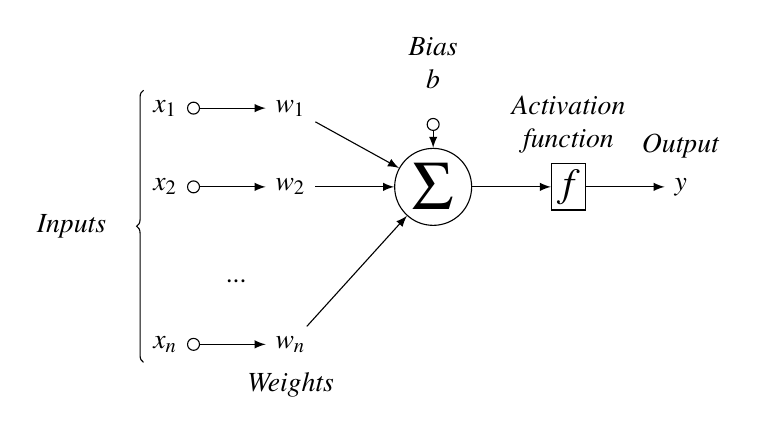
\begin{tikzpicture}[
init/.style={
  draw,
  circle,
  inner sep=2pt,
  font=\Huge\itshape,
  join = by -latex
},
squa/.style={
  draw,
  inner sep=2pt,
  font=\Large,
  join = by -latex
},
start chain=2,node distance=10mm
]
\node[on chain=2] 
  (x2) {$x_2$};
\node[on chain=2,join=by o-latex] 
  {$w_2$};
\node[on chain=2,init] (sigma) 
  {$\displaystyle\Sigma$};
\node[on chain=2,squa,label=above:{\parbox{2cm}{\centering \textit{Activation \\ function}}}]   
  {$f$};
\node[on chain=2,label=above:\textit{Output},join=by -latex] 
  {$y$};
\begin{scope}[start chain=1]
\node[on chain=1] at (0,1cm) 
  (x1) {$x_1$};
\node[on chain=1,join=by o-latex] 
  (w1) {$w_1$};
\end{scope}
\begin{scope}[start chain=3]
\node at (0.9, -1.2cm) (dots) {...};
\node[on chain=3] at (0,-2cm) 
  (x3) {$x_n$};
\node[on chain=3,label=below:\textit{Weights},join=by o-latex] 
  (w3) {$w_n$};
\end{scope}
\node[label=above:\parbox{2cm}{\centering \textit{Bias} \\ $b$}] at (sigma|-w1) (b) {};

\draw[-latex] (w1) -- (sigma);
\draw[-latex] (w3) -- (sigma);
\draw[o-latex] (b) -- (sigma);

\draw[decorate,decoration={brace,mirror}] (x1.north west) -- node[left=10pt] {\textit{Inputs}} (x3.south west);
\end{tikzpicture}}
	\caption{A model of an artificial neuron. \label{fig:artificial-neuron}}
\end{figure}


%\acp{ANN} were, however,  inspired by biological neural
%networks~\cite{kohonen1988introduction}, which produce recurrent spatio temporal patterns~\cite{rolston2007precisely}. 
%Similar timed activity of neurons in the cerebellum has been reported
%in~\cite{bullock1994neural}. 
%\ignore{Removed reference moore1989adaptively}
\acp{ANN} to be used
in CPS must be \emph{reactive}, meaning that they must operate in a
reactive loop.
In each loop, they will read their inputs,
then process this using the neural network, and at the end of the
loop emit the outputs. If the duration of this loop is bounded by a
fixed period, then we can produce outputs relative to the changes in
inputs in a periodic manner, which will ensure timely behaviour of
\ac{ANN}. Such neural networks are known as \acp{SNN}~\cite{sann}, which we
re-formalise by the following two definitions.

%\subsection{Motivating Example}

\subsection{Formalisation}

\begin{definition}
	\label{def:bb-mlp}
	Any stateless \ac{ANN} (e.g. \acp{MLP}, \acp{CNN}, etc) can be formalised as a tuple $M = \langle I, O, \lambda  \rangle$, where:
        \begin{itemize}
        \item $I$ is a finite collection of input variables with
          its domain being $\mathbf{I} =\mathbb{R}^n$
        \item  $O$ is a finite collection of  output variables with
          its domain being $\mathbf{O} = \mathbb{R}^m$
       % \item  $N$ denotes a set of neurons
        %\item $L$ denotes a set of layers
        %\item $\alpha: N \rightarrow L$ is the neuron mapping function
        % that maps a given neuron to a layer
         \item $\lambda: \mathcal{I} \rightarrow \mathcal{O}$ is the non-linear
          function (termed the network function) that provides the behaviour of a given neural network i.e.
          when provided a vector of input of size $n$ produces an
          vector of output of size $m$. 
        \end{itemize}
\ignore{
 $i \in I$ is each input to the network, $o \in O$ is each output from the network, 
$\eta$ is the set of neurons, $L$ is the set of layer functions $l:i \rightarrow o$ which perform intermediate data transforms, $m: \eta \rightarrow L$ is the neuron mapping function that associates a neuron to a given layer,
 and $f: I \rightarrow O$ is a function that captures the non-linear behaviour of the entire network 
--- i.e. a ``black-box'' untimed non-linear transformation function which converts inputs to outputs via the execution of each layer of neurons in sequence.}
%$m \subset \eta \times L$ provides the mapping of neurons to layers. 
%	We can describe the operation of $n$ as $n\left(I\right) = O$, i.e. $n$ describes a `black-box' untimed non-linear transformation function which converts inputs to outputs via the execution of each layer of neurons.
\end{definition} 

\begin{definition}%\footnote{While this section formalises \acp{MLP},
    %the proposed \ac{SNN} definition trivially extends %to other types
   % of neural networks such as \acp{CNN}.}
%	\label{def:bb-snn}

Given an \ac{ANN} $M = \langle I, O, \lambda  \rangle$, we
define a \ac{SNN} based on $M$ to be a periodic invocation of $\lambda$,
which requires one \emph{tick} to complete, where a tick
denotes the fixed period of a logical clock.
\end{definition}


\subsection{Run-Time Enforcement of \acp{SNN} using \acp{ENN}}

%\subsubsection{\acf{RE}}

\acf{RE} is a subset of \ac{RA} that focuses on making a system policy
compliant by modifying and/or re-ordering of events in a
system~\cite{theoryRE}. Initial techniques were designed for
\emph{transformational systems} where delaying events by buffering
is tolerable. As \ac{CPS} are reactive in nature, new methods have
been developed that enforce a set of timed policies by altering the
input / outputs suitably during the same reactive
cycle~\cite{RuntimeEnforcementOfCPS}. This approach is especially relevant for the
design of safe neural networks using \ac{RE}.

\ignore{formal semantics and blocking, delaying, modifying and/or re-ordering of events in a system. 
\ac{RE} can be transformation or reactive.
Transformational \ac{RE} uses the delaying, buffering and reordering of event to enforce a safety policy, while reactive \ac{RE} uses edit functions to edit events and can be bi-directional.
This paper focuses on reactive \ac{RE}, since \acp{ANN} are reactive in nature.

Processes that are deemed unsafe can be monitored by an enforcer at runtime to ensure that they obey desired policies and remain in a safe state at all times~\cite{theoryRE}. 
Formal runtime verification methodologies mathematically guarantee the detection of improper system behaviour \cite{RuntimeAssuranceForComplexCPS}.
For example, \ac{SA} have been proposed, which formally monitor uni-directional run-time properties only (e.g. outputs only)~\cite{enfsafepol}.
Edit automata are a type of \ac{SA} that can edit, suppress or insert events~\cite{editautomata}. 
\ac{DTA} have been proposed that can edit \textit{bi-directional} events at runtime~\cite{recps}. 
They were designed for reactive \ac{CPS} demonstrated in a pacemaker
environment~\cite{recps}.}

An \ac{ENN} is an extension of \ac{SNN} by adding an enforcement
layer, which suitably regulates the inputs from the plant and the
outputs generated by the \ac{SNN} every tick. The enforcement layer
consists of an \emph{input enforcer} that regulates the inputs $I$ every
tick to make them policy compliant. These transformed inputs $I'$ are
fed to the input layer of the \ac{SNN}. Once the \ac{SNN} produces its
output, either in the same or a future tick, an output enforcer may
transform the outputs $O$ to policy compliant outputs $O'$, which are
then fed to the plant. This reactive cycle repeats ad-infinitum. Also,
when the IO remain policy compliant, no changes are made by the enforcer.
Figure~\ref{fig:rebasic} shows the structure of a \ac{ENN}.

\begin{figure}[!htb]
	\centering
	\includegraphics[scale=1.0]{Content/fig/model-driven-ai-enns.pdf}
	\caption{Architecture of an enforced neural network}
	\label{fig:rebasic}
\end{figure}

\ignore{
\begin{figure}[!htb]
	\centering
	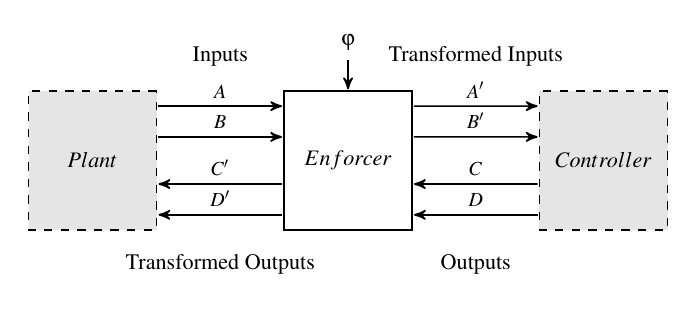
\begin{tikzpicture}[->, >=stealth', shorten >=0.15mm, shorten <=0.15mm, semithick, scale=0.8, transform shape]

\def\separation{20mm}

\tikzstyle{line} = [draw, -latex']

\tikzset{complete-box/.style={rectangle, draw, fill=none, minimum height=2.2cm, text width = 1.8cm, text centered}}

\tikzset{dashed-box/.style={complete-box, dashed, fill=black!10}}


\node[dashed-box]
(Plant) {$Plant$};

\node[complete-box, anchor=west] at ($ (Plant.east) + (\separation, 0) $)
(Enforcer) {$Enforcer$};

\node[dashed-box, anchor=west] at ($ (Enforcer.east) + (\separation, 0) $)
(Controller) {$Controller$};

\node [above = 0.25*\separation of Enforcer.north] (prop) {$\varphi$};


\node [anchor=south] at ($ (Plant.north east) + (0.5*\separation, 0.125*\separation) $) (inputsLabel) {Inputs};

\node [anchor=south] at ($ (Enforcer.north east) + (0.5*\separation, 0.125*\separation) $) (transformedInputsLabel) {Transformed Inputs};

\node [anchor=north] at ($ (Enforcer.south east) + (0.5*\separation, -0.125*\separation) $) (outputsLabel) {Outputs};

\node [anchor=north] at ($ (Plant.south east) + (0.5*\separation, -0.125*\separation) $) (transformedOuputsLabel) {Transformed Outputs};


\draw[->] (Plant.40) -- node[above] { \small $A$ } (Enforcer.140);
\draw[->] (Plant.20) -- node[above] { \small $B$ } (Enforcer.160);
\draw[->] (Enforcer.200) -- node[above] { \small $C'$ } (Plant.340);
\draw[->] (Enforcer.220) -- node[above] { \small $D'$ } (Plant.320);

\draw[->] (Enforcer.40) -- node[above] { \small $A'$ } (Controller.140);
\draw[->] (Enforcer.20) -- node[above] { \small $B'$ } (Controller.160);
\draw[->] (Controller.200) -- node[above] { \small $C$ } (Enforcer.340);
\draw[->] (Controller.220) -- node[above] { \small $D$ } (Enforcer.320);

\draw[->] (prop.south) -- (Enforcer.north);


\end{tikzpicture}

	\caption{Architecture of an enforced neural network}
	\label{fig:rebasic2}
\end{figure}
}

%\subsection{Synchronous Neural Networks}


%\subsection{Meta Neural Networks}

\subsection{Methodology and Assumptions}

The design of \acp{ENN} is performed as follows. The Esterel~\cite{Berry00}
synchronous programming language is used for the implementation of
\acp{SNN}. We can use existing C-based libraries such as
Darknet~\cite{darknet13} to create neural networks during the learning
phase. Once the learning phase is completed, we can create C-functions
with associated header files which store the weights. These can then be
invoked as \texttt{host-functions} in Esterel to create an individual \ac{SNN}. 

Esterel also provides an excellent avenue to create complex
applications using  \emph{synchronous concurrency}. This enables
several \acp{SNN} to be composed synchronously to
create neural network ensembles~\cite{Maqsood2004}, which are very useful in
creating complex AI applications that combine \acp{CNN} with other
types of \acp{ANN} in a systematic way. 

A given ensemble becomes a synchronous program, which can be combined
with other synchronous components easily in Esterel as the composition
of synchronous modules. We use this to combine the controller
represented as a neural network ensemble with the enforcer. Finally,
the overall system is composed with the reactive environment using the
standard approach of reactive interfaces. As Esterel programs are
automatically compiled to a single reactive function in C, where all
concurrency is ``compiled away'', the generated code is WCET
analysable, as shown in~\cite{sann}. However, this part is outside the
scope of the current work.
%\section{Background}
%%Hammond / Srinivas -- you may change the following if you think of a better structure

\ignore{
\subsubsection{\acf{RV}}
Run-time verification is an extension of run-time monitoring~\cite{runtime-verify}.
A run-time verifier monitors the I/O events of a system using a specified safety policy.
The verifier provides positive or negative feedback depending on the I/O of the system, providing a verdict for the current state of the automaton.
The run-time verifier has no knowledge of the inner workings of the system, regarding it as a black box.
This makes it ideal for autonomous systems, where the inner workings are often too complex to be verified.

\subsubsection{\acf{RE}}

\acf{RE} is a subset of \ac{RA} that focuses on formal semantics and blocking, delaying, modifying and/or re-ordering of events in a system. 
\ac{RE} can be transformation or reactive.
Transformational \ac{RE} uses the delaying, buffering and reordering of event to enforce a safety policy, while reactive \ac{RE} uses edit functions to edit events and can be bi-directional.
This paper focuses on reactive \ac{RE}, since \acp{ANN} are reactive in nature.

Processes that are deemed unsafe can be monitored by an enforcer at runtime to ensure that they obey desired policies and remain in a safe state at all times~\cite{theoryRE}. 
Formal runtime verification methodologies mathematically guarantee the detection of improper system behaviour \cite{RuntimeAssuranceForComplexCPS}.
For example, \ac{SA} have been proposed, which formally monitor uni-directional run-time properties only (e.g. outputs only)~\cite{enfsafepol}.
Edit automata are a type of \ac{SA} that can edit, suppress or insert events~\cite{editautomata}. 
\ac{DTA} have been proposed that can edit \textit{bi-directional} events at runtime~\cite{recps}. 
They were designed for reactive \ac{CPS} demonstrated in a pacemaker environment~\cite{recps}. 
Figure~\ref{fig:rebasic} shows the structure of a basic bi-directional run-time enforcer over controller inputs $\{A,B\}$ and controller ouptuts $\{C,D\}$.

\begin{figure}[!htb]
	\centering
	\includegraphics[scale=1.1]{Content/fig/enforced-snns.pdf}
	\caption{Generalised bi-directional enforcer.}
	\label{fig:rebasic}
\end{figure}
}

\section{Motivating Example}
\label{sec:av-casestudy}
%Here we present the overview of the proposed approach that combines SNNs with RE i.e. \acfp{ENN}.
%We also present the case study.

%\subsection{Case Study: \acf{AV}}
%\label{sec:av-casestudy}
\acfp{AV} are \acf{CPS} that are safety critical as highlighted by
recent fatalities involving Tesla and Uber \acp{AV}~\cite{coldewey_2018}~\cite{stewart_2018}.
In this paper, we take inspiration from such accidents and create a case study involving the braking mechanism of \acp{AV}.

\begin{figure}[h]
	\centering
	\includegraphics[scale=0.24,trim={0 7mm 0 7mm},clip ]{Content/fig/AV.pdf}
	\caption{Sensor layout for the \ac{AV} example. \label{fig:av}}
\end{figure}
\vspace{1em}
The abstracted \acf{AV} is represented in Figure~\ref{fig:av} .
It will manage forward linear movement of the \ac{AV} and the braking involved with such movement.
The simulation environment consists of one \ac{AV} interacting with other vehicles and pedestrians in its proximity.
The \ac{AV} is run by an autonomous controller with 5 directional sensor inputs, each of which is a camera with its own field of view.
Each camera also features a \acf{LiDAR} sensor for detecting the
distance and shapes of objects in its vicinity.
Each of the five cameras feeds into a \acf{MNN} ensemble~\cite{Maqsood2004} of \acp{SNN}, using the Darknet library~\cite{darknet13}, while the \ac{LiDAR} readings are passed directly to the controller.
\begin{figure}[b]
	\centering
	\includegraphics[scale=1.0]{Content/fig/model-driven-ai-av-example.pdf}
	\caption{Block diagram of \ac{ENN} system used in \ac{AV} case study. \label{fig:avnenf}}
	\vspace{-4mm}
\end{figure}

An \ac{ANN} ensemble is created by execution of multiple \acp{ANN} working in tandem to produce more accurate output~\cite{Maqsood2004}.
%An ensemble can contain different \acp{ANN}, with different structures, inputs, outputs and even programming languages.
%The output of an \ac{ANN} ensemble represents some combination of all the \acp{ANN} in the ensemble, and is more accurate than any individual \ac{ANN} in the ensemble.
These \ac{SNN} ensembles classify their input image and provide a confidence level for the classified image, before passing this information to the controller.
The controller \ac{SNN} is a \ac{MLP}, and decides the best course of action given the environment and the status of the vehicle. 
\ignore{
The current status of the vehicle is noted by the current speed of the
vehicle ($S$) and the previous speed of the vehicle($S'$) obtained in
the previous \emph{tick}.
The controller then outputs one of three commands to the actuators.
These commands are as follows: accelerate ($A$); brake softly ($B_S$);
and brake hard ($B_H$).~\pr{Now our policy allows progressive braking}
}
A block diagram of the \ac{AV} used in this system is shown in Figure~\ref{fig:avnenf}. 


\ignore{
\subsection{Case Study: \acf{ESS}} \label{sec:ess4}
The \ac{ESS} is inspired by \cite{chaudhari2017hybrid}, in which an \ac{EV} charging station has a separate battery that it uses to assist the charging of the \acp{EV}, with the general idea that the battery is charged when power is cheap, and discharged when demand is high or power is expensive.
The \ac{ESS} uses a pre-trained, three-layer \ac{MLP} to decide the action for the battery in the next tick.
While the \ac{AV} system is a hard real-time system the \ac{ESS} system is a soft real-time system, as a missed deadline will not result in fatalities.
Failures in this system could cause damage to electrical components and potentially cause fires (from overcharging or overcurrent) and maybe even customer property, i.e. the charging station and the \acp{EV}, and thus appropriate policies can be put into place to make the system safer.
\ac{RE} can be used to formally guarantee that the controller will behave safely at all times.
Systems with \acp{ANN} are difficult to verify.
\ac{RE} can ensure that they behave safely even in the event of unexpected inputs.
The enforced policies monitor the controller's \ac{MLP} outputs and ensure that (1) the battery levels never reach critical levels, and (2) that too much power is never given or taken from the battery in too short a period of time.
Running this system with enforced policies shows that the battery's \ac{SoC} never exceeds critical values and that the battery never charges or discharges too much power.
The charge of buying and selling electricity to the customer's \ac{EV} does not change by any significant amount when the enforcer is in place, i.e. it does not affect the performance of the system while it keeps the system safe.}

\section{Valued Discrete Timed Automata}
%In this section, we firstly present some preliminaries and notations
%used. Later we describe the syntax and semantics of the Valued
%Discrete Timed Automata (VDTA).
 We propose \acf{VDTA} to formally represent properties,
 from which enforcement monitors are synthesized. We start with a
 motivating example.

%\todo{This has been lifted from TII and should be rephrased where possible. Examples will be updated of course.}
%\subsection{Preliminaries}
%\todo{SP: added the following paragraph.}
%\red{
%	
%A finite (resp. infinite) word over a finite alphabet $\Sigma$ is a finite sequence $\sigma = a_1\cdot a_2\cdots a_n$ (resp. infinite sequence $\sigma = a_1\cdot a_2\cdots$) of elements of $\Sigma$.
%The set of finite (resp. infinite) words over $\Sigma$ is denoted by $\Sigma^*$ (resp. $\Sigma^\omega$).
%The {\em length} of a finite word $\sigma$ is $n$ and is denoted by $|\sigma|$.
%The empty word over $\Sigma$ is denoted by $\epsilon_\Sigma$, or $\epsilon$ when clear from the context.
%$\Sigma^+$ denotes $\Sigma^*\setminus\{\epsilon\}$.
%The {\em concatenation} of two words $\sigma$ and $\sigma'$ is denoted by $\sigma\cdot \sigma'$.
%A word $\sigma'$ is a {\em prefix} of a word $\sigma$, denoted as $\sigma' \pref \sigma$, whenever there exists a word $\sigma''$ such that $\sigma = \sigma'\cdot \sigma''$; conversely $\sigma$ is said to be an \emph{extension} of $\sigma'$.
%}


\begin{figure}[t]
	\centering
	\input{./Content/fig/av-ped-rte-small}
	\caption{Simplified pedestrian safety policy $\mathcal{A}_{ped}$}
	\label{fig:vdta-car-rte}
\end{figure}

\begin{example}
	\label{eg:vdta}
	%we need values because of tau
	%deadline is a function of the overcurrent value
	
	A pedagogic simplification of pedestrian safety policy is a \ac{VDTA} $\mathcal{A}_{ped}$, as
        depicted in Figure~\ref{fig:vdta-car-rte}.
        The complex policy is used in Section~\ref{sec:resultsc4}.
	%While in reality this is a very complex policy, as the process of detecting a pedestrian relies on processing the data from multiple sensors, we have simplified it in this section for pedagogical purposes.
	%This is a policy involving both valued and timed properties, as follows.
	Assume that we have the input $P$, which represents the distance (in metres) from the car to the nearest pedestrian.
	$P$ is a value from $0$ to $100$ to indicate a valid distance, or $101$ to indicate no pedestrian in range.
	
	In response to a pedestrian at distance $P$, within one tick
        the car should apply brakes by setting the value the actuator
        $B$ as a percentage of maximum braking effort.
	We define function $br: P \rightarrow B$, which takes a
        pedestrian distance $P$ and returns the value of $B$ using $br\left(P\right) = \big(\frac{100 - P}{100}\big)$. 
	Thus, the braking pressure increases linearly based on the distance to the pedestrian. To ensure safety, the car must always apply brakes for a minimum period of time, which we call $T_{lim}$.
	
	%However, due to perturbations in sensory data, the detection methodology for the pedestrian may oscillate around the true value.
	
	%As a result, if a pedestrian is detected, the system should \emph{fail-safe}.
	%To do this, 
	
\end{example}

A VDTA can be seen as an automaton with a finite set of locations, a
finite set of discrete clocks used to represent time evolution, and
external input (resp. output channels) called ``external variables''
which are used for representing system data.They model the data from
the monitored system (resp. environment) read from the input (resp.)
channels in every tick. 
In a \ac{VDTA}, time evolves synchronously: that is, the system executes as a series of discrete \emph{logical ticks} where each tick takes exactly one transition~\cite{SynchronousLanguages12YearsLater}.
In the semantics of VDTA, each transition will be associated with values of external variables.
%They also have internal variables which are used for internal computation, compared to the external variables which model the data carried by the actions from the monitored system (resp. environment). 

\ignore{
Within \ac{VDTA}, there is an implicit logical tick similar to synchronous programming languages
All transitions occur relative to this tick.
At the start of a tick, all input channels are sampled, and at the end of the tick, all output channels are emitted.
Thus, a tick constitutes and atomic reaction of the reactive system.
}

%On transition edges, variables (input and output channels) are updated.
%Static timing analysis techniques can be used to compute .

	
	%	The \ac{VDTA} has a set of actions $\Sigma = \{tk(i, i_{set}, r)\}$.
	%	It consists of only a default ``tick'' action, which represents the ticking of a ``logical clock'' called ``tk''. 
	%	In every tick, the values of all input-output channels are updated.
	
%\end{example}

\subsection{Syntax and Semantics}
We consider our Cyber-Physical Systems to have finite ordered sets of valued input channels ${I} = \{{i_1}, {i_2}, \ldots {i_n}\}$ and valued output channels ${O} = \{{o_1}, {o_2}, \ldots {o_n}\}$.
%Before we look into the formal definition of VDTA, let us consider an example.
%Let us now consider in more detail the syntax and semantics of VDTAs.
%
For a variable (resp. channel) $v$, ${\mathcal D}_v$ denotes its domain,
and for a finite ordered set of variables $V= \{v_1, \ldots, v_n \big\}$,
${\mathcal D}_V$ is the product domain ${\mathcal D}_{v_1} \times \cdots \times {\mathcal D}_{v_n}$.
%A predicate $P(V)$ on a tuple of variables $V$ is a logical formula whose semantics is a function ${\mathcal D}_V \rightarrow \{\true, \false\}$.
A valuation of the variables in $V$
is a mapping $\nu$ which maps every variable $v \in V$ to a value $\nu\big(v\big)$ in ${\mathcal D}_v$.
%
Let $X=\{x_1,\ldots, x_k\}$ be a finite set of integer variables representing discrete clocks.
%
A {\em valuation} for $x$ is an element of $\bbn$, that is a function from $x$ to $\bbn$.
The set of valuations for the set of clocks $X$ is denoted by $\chi$.
%
For $\chi\in\bbn^X$, $\chi+1$ (which captures the ticking of the digital clock) is the valuation assigning $\chi\left(x\right)+1$ to each clock variable $x$ of $X$.
Given a set of clock variables $X' \subseteq X$, $\chi\left[X' \leftarrow 0\right]$ is the valuation of clock variables $\chi$ where all the clock variables in $X'$ are assigned to $0$.


%
\begin{definition}[Syntax of {VDTA}s]
	\label{def:ptav}
	A {VDTA} is a tuple \\
	$\calA = \left(L, {l_0}, X, C, F,  \Delta \right)$ where:
	\squishlist
	%	\item $\Sigma$ is a non-empty finite set of actions,
	%	and an action $a \in \Sigma$ has a signature $sig(a) = ( t_0, t_1, \ldots, t_k )$ which is a tuple of types of the external variables,
	\item $L$ is a finite non-empty set of locations, with $l_0 \in L$ the initial location, and $F \subseteq L$ the set of accepting locations;
	\item $X$ is a finite set of discrete clocks;
	%\item $V$ is a tuple of typed internal variables; 
	\item $C$ is a tuple of external variables, where $C = I \cup O$, where $I$ is the set of input channels, and $O$ is the set of output channels; 
	%\item $\Theta\subseteq {\mathcal D}_{V }$ is an initial condition which is a computable predicate over $V$;
	\item $\Delta$ is a finite set of transitions, and each transition $t \in \Delta$ is a tuple $\left( l, G, A^X, l' \right)$
	also written\\
	$l \xrightarrow{G\left( C \right),A^X} l'$
	such that,
	\squishlist
	\item[\textbullet] $l, l' \in L$ are respectively the origin and target locations of the transition;
	%\item[\textbullet] $c$ is a tuple of external variables;
	\item[\textbullet] $G = G^D \wedge G^X$ is the guard where
	\squishlist
	\item[-] $G^D$ 
	is a computable predicate over external variables  in $C$;
	\item[-] $G^X$ is a clock constraint over $X$ defined as conjunctions of constraints of the form $x \sharp f\left(C\right)$, where $x \in X$ and $f\left(  C \right)$ is a computable function, and $\sharp \in \{ <, \leq, =, \geq, > \}$;
	\squishend
	\item[\textbullet] $A^X \subseteq X$ is the set of clocks to be reset.
	%\item[\textbullet] $A$$=$$(A^D, A^X)$ is the assignment of the transition where
%	\squishlist
	%\item[-] $A^D :{\mathcal D}_V  \rightarrow {\mathcal D}_V$ defines the evolution of internal variables.
	
%	\squishend
	\squishend
	\squishend
\end{definition}
%

\begin{example}	
	
	The \ac{VDTA} for Figure~\ref{fig:vdta-car-rte} has a set of
        locations $L = \{ l_{safe},l_{brake}, l_{v}\}$, with accepting
        locations F = $\{l_{safe}\}$. $l_{safe}$ is also the initial
        location.
	The \ac{VDTA} has the set of external variables  $C = \{P,
        B\}$, where $P$ is an input real-valued channel, 
        and $B$ is an output real-valued channel.
	
	In a VDTA, a transition can have guards on  external variables and clocks. 
	For example, the transition from $l_{safe}$ to $l_{brake}$
        happens when $P \leq 100$. 
	The clock values can be reset upon transitions. 
        For example, upon transition from $l_{safe}$ to $l_{brake}$, the value of clock $t$ is reset to 0.
        
    After a pedestrian is detected, a transition from location $l_{safe}$
    to $l_{brake}$ is taken. 
    Here it must remain as long as two conditions are met.
    Firstly, pedestrian $P$ is within 100 metres.
    Secondly, time $t$ is less than than $T_{lim}$.
    
    There is one violation transition, from $l_{brake}$ to $l_v$. 
    This occurs when either the brakes are not pressed hard enough while the
    pedestrian is within collision range, or if the pedestrian was detected less than $T_{lim}$ time units ago yet the controller has already stopped braking.
\end{example}
%A word is a sequence $\sigma = \eta_1\cdot \eta_2 \cdots \eta_n$ where $\forall i \in [1,n]:$ $\eta_i$ is a tuple of values of variables in $C = I \cup O$.
	
A finite (resp. infinite) word over $\calD_C$ (where $C = I \cup O$) is a finite sequence $\sigma = \eta_1\cdot \eta_2 \cdots \eta_n$ where $\forall t \in [1,n]:$ $\eta_t$ is a tuple of values of variables in $C = I \cup O$. For convenience where necessary, each element $\eta_i$ is considered to be a pair $\left(\eta_I, \eta_O\right)$, where $x_i$ is a valuation of all the variables in $I$, and   $y_i$ is a valuation of all the variables in $O$.
The set of finite (resp. infinite) words over $\calD_C$ is denoted by $\calD_C^*$ (resp. $\calD_C^\omega$).
The {\em length} of a finite word $\sigma$ is $n$ and is denoted by $|\sigma|$.
The empty word over $\calD_C$ is denoted by $\epsilon_C$, or $\epsilon$ when clear from the context.
$\calD_C^+$ denotes $\calD_C^*\setminus\{\epsilon\}$.
The {\em concatenation} of two words $\sigma$ and $\sigma'$ is denoted by $\sigma\cdot \sigma'$.
A word $\sigma'$ is a {\em prefix} of a word $\sigma$, denoted as $\sigma' \pref \sigma$, whenever there exists a word $\sigma''$ such that $\sigma = \sigma'\cdot \sigma''$; conversely $\sigma$ is said to be an \emph{extension} of $\sigma'$.

A property $\varphi$ over $C$ defines a set $\calL\left(\varphi\right)\subseteq \calD_C^{*}$.
A program $\calP \models \varphi$ iff $\calL\left(\calP\right) \subseteq  \calL\left(\varphi\right)$.
In this paper, properties are formally defined as VDTA.

%Policy \ac{VDTA} are required to be \textit{deterministic}, i.e. for any given state, the conjunction of any guards of any other outgoing transitions may not be satisfiable; and \textit{complete}, i.e. for any given state at any given time and any valuation of variables in $C$, at least one transition guard is satisfied.

\subsubsection{Semantics for \ac{VDTA}}

Let $\calA = \left(\Sigma, L, {l_0}, X, C, F,  \Delta \right)$  be a VDTA.
The semantics of $\calA$ is a timed transition system,
where a state consists of a location, and valuations of clocks $X$.
Each transition is associated with values of external variables in $C$.

\begin{definition}[Semantics of {VDTA}s]
	\label{def:vdta:semantics}
	The semantics of $\calA$ is a timed transition system $\sem{\calA}=\left( Q, q_0, Q_F, \Gamma, \to \right)$, defined as follows:
	\squishlist
	\item $Q = L \times \bbn^X$, is the set of states of the form $q= \left( l,\chi \right)$ where
	$l \in L$ is a location,
%	$\nu \in {\mathcal D}_V$ is a valuation of internal variables,
	$\chi$ is a valuation of clocks;
	\item $Q_0 = \{ \left( l_0, \chi_{\left[X \leftarrow 0\right]} \right) \}$ is the set of initial states;
	\item $Q_F = F \times  \bbn^X$ is the set of accepting states;
	\item $\Gamma = \{ \eta \mid
	\eta \in {\mathcal D}_{C}  \}$ is the set of transition labels;
	\item $\to\subseteq Q\times \Gamma\times Q$  the transition relation
	is the smallest set of transitions of the form
	$\left( l,\chi \rangle \longrightarrow {\eta} \langle l',\chi'\right)$
	such that  $\exists \left( l, G, A^X, l' \right) \in \Delta$,
	with $G^X\left(\chi + 1\right) \wedge G^D\left(\eta\right) $ evaluating to {\true},
	%$\nu'= A^D\left(\nu\right)$ 
	and $\chi'=\left(\chi+1\right)[A^X \leftarrow 0]$.
	\squishend
\end{definition}

A {\em run} $\rho$ of $\sem{\calA}$ from a state $q\in Q$ over a {\em trace} $w =  \eta_1\cdot \eta_2\cdots \eta_n$ is a sequence of moves in $\sem{\calA}$:
$\rho = q \xrightarrow {\eta_1} q_1
\cdots q_{n-1}\xrightarrow {\eta_n} q_{n}$,
for some $n\in\bbn$.
A run is accepted if it starts from the initial state $q_0\in Q$ and ends in an accepted state $q_n \in Q_F$.
%The set of runs from the initial state $q_0\in Q$,  is denoted $\Run(\calA)$ and $\Run_{Q_F}(\calA)$ denotes the subset of those runs {\em accepted} by $\calA$, i.e.,  ending in an accepting state $q_n \in Q_F$.

%%%%%%%%%%%%%%%%%%%%%%%%%%%%%%%%%%%%%%%%%%%%%%%
%%%%%%%%%%%%%%%%%%%%%%%%%%%%%%%%%%%%%%%%%%%%%%%
\begin{example}[Run of a VDTA]
	%Let us consider the VDTA %discussed in Example~\ref{eg:vdta}
	%presented in Figure~\ref{fig:vsa-overcurrent}. 
	An example run of the VDTA depicted in Figure~\ref{fig:vdta-car-rte} is elaborated here.
	Assume $T_{lim} = 5$.
	A run of this VDTA starting from the initial state $\left(l_{safe}, t = 0\right)$ for the word $\sigma = \left(101,0\right)\cdot \left(100,0\right)\cdot \left(90,0.2\right)\cdot \left(101,0.2\right)\cdot\left(75,0.4\right)\cdot \left(70,0\right)$ is:\\
	{\small$
		\left(l_{safe}, t = 0\right)
		\xrightarrow {\left(101, 0\right)} 
		\left(l_{safe}, t = 1\right)
		\xrightarrow {\left(100, 0\right)} 
		\left(l_{brake}, t = 0\right)
		\xrightarrow {\left(90, 0.2\right)} \\
		\left(l_{brake}, t = 1\right)
		\xrightarrow {\left(101, 0.2\right)} 
		\left(l_{brake}, t = 2\right)
		\xrightarrow {\left(75, 0.4\right)} 
		\left(l_{brake}, t = 3\right)
		\xrightarrow {\left(70, 0\right)} 
		\left(l_{vio}, t = 4\right).
		$
	}
	
	The run started in the initial state.
	A pedestrian is detected in the second tick, and in the third tick, the \ac{AV} starts braking with $B = 0.2$. 
	This meets the safe threshold.
	In the fourth tick, the input sensor package misclassifies and says that no pedestrian is detected, setting $P = 101$.
	However, the controller continues to brake with $B = 0.2$.
	The pedestrian is re-detected in the fifth tick and the car continues to brake.
	However, in the sixth tick, the controller malfunctions, and even though a pedestrian is still detected, it stops braking.
	As a result, the \ac{VDTA} will go to the non-accepting state $l_v$. 
	This is thus a non-accepting run and represents a violation scenario.
\end{example}
%%%%%%%%%%%%%%%%%%%%%%%%%%%%%%%%%%%%%%%%%%%%%%%%%%%%%%%%%%
\begin{definition}[Deterministic (complete) \ac{VDTA}]
	\label{def:detComplete}
	A VDTA $\calA= \left(L, {l_0}, X, C, F,  \Delta \right)$ with its semantics $\sem{\calA}$ is said to be a {\em deterministic} \ac{VDTA} whenever for any location $l$
	and any two distinct transitions $\left(l,g_1,A^X_1,l'_1\right) \in \Delta$ and $\left(l, g_2, A^X_2, l'_2 \right)\in \Delta$ with same source $l$, the conjunction of guards $g_1\wedge g_2$ is unsatisfiable.
	$\calA$ is {\em complete} whenever for any location $l\in L$ the disjunction of the guards of the transitions leaving $l$ evaluates to {\em true}.
\end{definition}

%%%%%%%%%%%%%%%%%%%%%%%%%%%%%%%%%%%%
\ignore{
\begin{definition}[Product of VDTAs]
	\label{VDTA:product}
	Given two VDTAs 
		\[\calA^{1} = \left(L^{1}, {l_0}^{1}, X^{1}, V^{1}, C^{1}, \Theta^{1}, F^{1},  \Delta^{1} \right)\] and
		\[\calA^{2} = \left(L^{2}, {l_0}^{2}, X^{2}, V^{2}, C^{2}, \Theta^{2}, F^{2},  \Delta^{2} \right)\]
		with disjoint sets of integer clocks (X), internal variables (V) and external variables (C), their product is the VDTA \[\calA^{1}\times \calA^{2}= \left(L, {l_0}, X, V, C, \Theta, F,  \Delta \right)\] where
	$L=L^1 \times  L^2$, $l_0 = (l^1_{0}, l^2_{0})$,  $X  = X^1 \cup X^2$  , $V  = V^1 \cup V^2$ ,  $C  = C^1 \cup C^2$, $F = F^1 \times F^2$, 
 $\Theta = \Theta^{1} \wedge \Theta^{2}$
	and  $\Delta$ 
	is a finite set of transitions where each transition $t=\left( \left(l^{1},l^{2}\right), G^{1}\wedge G^{2}, A^{1} \cup A^{2}, \left(l^{'1},l^{'2}\right) \right)$ belongs to $\Delta$ if $\left( l^{1}, G^{1}, A^{1},l^{'1} \right)$ belongs to $\Delta^{1}$ and  $\left(l^{2}, G^{2}, A^{2},l^{'2} \right)$ belongs to $\Delta^{2}$.
\end{definition}

The product of \acp{VDTA} is useful when we have multiple properties to enforce.
}
%Given two  deterministic and complete \acp{DTA} $\calA^1$ and $\calA^2$ the \ac{DTA} $\calA$ obtained by computing their product recognizes the language $\calL(\calA^1) \cap \calL(\calA^2)$, and is also deterministic and complete.
%%%%%%%%%%%%%%%%%%%%%%%%%%%%%

\subsection{Edit Functions}
\label{sec:editfunc}
The proposed enforcement mechanism is allowed to edit input (resp. output) channels when necessary.
The edit functions that we introduce here will be used in defining the enforcer and  enforcement algorithm in the later sections. 
%%%%%%%%%%%%%%%%%%%%%%%%%%%%

In this framework it is possible to express bi-directional enforcement policies, where
the enforcer has to first transform inputs from the environment in each step according to property $\varphi$ defined as DTA $\calA_\varphi$.
We thus need to consider the input property that we obtain from $\calA_\varphi$ by projecting on inputs.

\begin{remark}[Input \ac{VDTA} $\calA_{I}$]
	\label{def:inp:prop:proj:def}
	Given a property defined as \ac{VDTA} $\calA=\left(L, {l_0}, X, C,  F,  \Delta \right)$, input \ac{VDTA} $\calA_{I}=\left(L, {l_0}, X,  C,  F,  \Delta_I \right)$ is obtained from $\calA$ by ignoring outputs channels on the transitions. For every transition $t \in \Delta$ there will be a transition $t' \in \Delta_I$ where $t' = \left( l, G', A'^X, l' \right)$ is obtained from t = $\left( l, G, A^X, l' \right)$ by discarding all the atomic formulas in $G^{D}$ and $G^{X}$ (which are both Boolean combination of formulas) that has output channels.
	\end{remark}
%
%\begin{definition}[Input \ac{VDTA} $\calA_{I}$]
%	\label{def:inp:prop:proj:def}
%	Given a property defined as \ac{VDTA} $\calA=\left(L, {l_0}, X, C,  F,  \Delta \right)$, input \ac{VDTA} $\calA_{I}=\left(L, {l_0}, X,  C,  F,  \Delta_I \right)$ is obtained from $\calA$ by ignoring outputs channels on the transitions. For every transition $t \in \Delta$ there will be a transition $t' \in \Delta_I$ where $t' = \left( l, G', A', l' \right)$ is obtained from t = $\left( l, G, A, l' \right)$ as follows:
%	\begin{itemize}
%		\item $G' = G^{D'} \wedge G^{X'}$, where  $G^{D'}$ and  $G^{X'}$ are obtained from $G^{D}$ (resp. $G^{X}$) by discarding any disjunct that has an output channel.  
%	\end{itemize}
%\end{definition}




In every tick, the enforcer has to first observe all the input channel values (and edit them if necessary), before it can observe and validate the values of the output channels.  
Input VDTA $\calA_I$  described in remark \ref{def:inp:prop:proj:def} is a property of inputs (only) that we obtain from a VDTA $\calA$ that expresses a property over both inputs and outputs. 
Input \ac{VDTA} may be non-deterministic.


\begin{figure}[tb]
	\centering
	

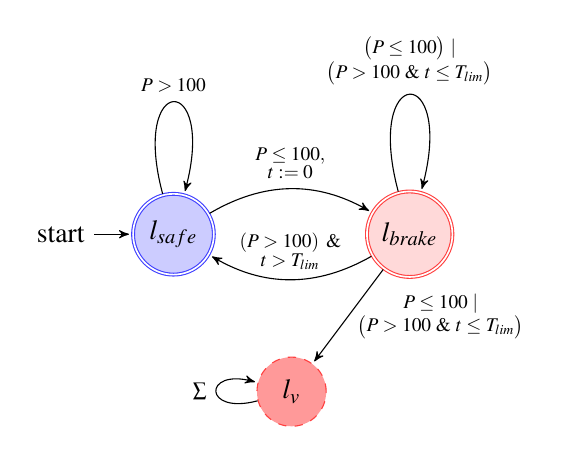
\begin{tikzpicture}[>=stealth',shorten >=1pt,auto,node distance=3 cm, scale = 1, transform shape]

\tikzstyle{accept} = [draw=blue!75,fill=blue!20]
\tikzstyle{violate} = [draw=red!75,fill=red!40, dashed]
\tikzstyle{unstable} = [draw=red!75,fill=red!15]

\node[state, initial, accepting, accept] (A) {$l_{safe}$};
\node[state, accepting, accept, unstable] (B) [right of=A] {$l_{brake}$};
\node[state, violate]         (C) [below of=B, yshift=1cm, xshift=-1.5cm]  {$l_v$};

\path[->] 
(A) edge [loop above,looseness=15]       node [above]  
{
	\scriptsize$\let\scriptstyle\textstyle\substack{P > 100}$
} (A)

(A) edge [bend left]		node [above]  
{
	\scriptsize$\let\scriptstyle\textstyle\substack{P \leq 100, \\ t := 0}$
} (B)

(B) edge [loop above,looseness=15]		node [above]  
{
	\scriptsize$\let\scriptstyle\textstyle\substack{\big(P \leq 100\big)~|\\\big(P > 100~\&~t\leq T_{lim}\big)}$
} (B)

(B) edge [bend left]				node [above]  
{
	\scriptsize$\let\scriptstyle\textstyle\substack{\left(P > 100\right)~\& \\ t > T_{lim}}$
} (A)

(B) edge [left]			node [right, xshift=0em]  
{
	\scriptsize$\let\scriptstyle\textstyle\substack{P \leq 100~|\\
		\big(P > 100~\&~t \leq T_{lim}\big)}$
} (C)

(C) edge [loop left]		node [left]  
{
	\scriptsize$\sum$
} (C)

;

\end{tikzpicture}
	\caption{Input VDTA $\mathcal{A}_{ped_I}$ obtained from $\mathcal{A}_{ped}$ in Figure \ref{fig:vdta-car-rte}}
	\label{fig:inp-vdta-car-rte}
	\vspace{-5mm}
\end{figure}

%%%%%%%%%%%%%%%%%%%%%%%%%%%%%
\begin{example}[Input \ac{VDTA} $\calA_{I}$ obtained from $\calA$]
Let us consider the \ac{VDTA} in Figure~\ref{fig:vdta-car-rte} defining the property introduced in Example~\ref{eg:vdta}.
Figure~\ref{fig:inp-vdta-car-rte} presents the input \ac{VDTA} obtained from the \ac{VDTA} in Figure~\ref{fig:vdta-car-rte}.
The violation transition $l_v$ need never be taken, as its guard is also satisfied by the self-loop on $l_{brake}$. 
As a result, $\mathcal{A}_{ped_I}$ will accept all runs, implying $\mathcal{A}_{ped}$ is a uni-directional policy.
\end{example}
%%%%%%%%%%%%%%%%%%%%%%%%%%%%
%%%%%%%%%%%%%%%%%%%%%%%%%%%%%
\paragraph{Edit Functions}
Given property $\varphi\subseteq \calD_C^*$, defined as \ac{VDTA} $\calA_{\varphi}=\left(L, {l_0}, X, C,  F,  \Delta \right)$ with semantics $\sem{\calA_\varphi}=\left( Q, q_0, Q_F, \Gamma, \to \right)$,
%we define and use the following:
we introduce $\editI$ (resp. $\editO$), which the enforcer uses for editing input (resp. output) events (whenever necessary), according to input property $\varphi_I$ (resp. input-output property $\varphi$).
Note that in each step the enforcer first processes the input from the environment, and transforms it using $\editI$ based on the input property $\varphi_I$ obtained from the input-output property $\varphi$ that we want to enforce.
Later, the output produced by the program is transformed by the enforcer (when necessary) using $\editO$ based on the input-output property $\varphi$ that we want to enforce.
%
\squishlist
\item {{\boldmath$\editI\left(\sigma_I\right)$}}:~~Given $I$ (set of input channels), $\editI\left(\sigma_I\right)$ is the set of all possible valuations $\eta_I$ (where $\eta_I$ is a tuple of values of variables in $I$) such that the word obtained by extending $\sigma_I$ with $\eta_I$ can be extended to a sequence that satisfies $\varphi_I$ (i.e., there exists $\sigma'\in \calD_I^*$ such that $\sigma_I\cdot \eta_I \cdot \sigma'$ satisfies $\varphi_I$).
Formally,\\
\[\editI\left(\sigma_I \right) = \{ \eta_I \in \calD_I: \exists \sigma'\in \calD_I^*, \sigma_I \cdot \eta_I \cdot \sigma' \models \varphi_I \}.\]
%Formally, \[\editI(\sigma_I) = \{ x\in \Sigma_I: \sigma_I \cdot x \models \varphi_I \}.\]

Consider the automaton
 $\calA_{\varphi_I}=\left(L, {l_0}, X,  C, F,  \Delta_I \right)$ with semantics $\sem{\calA_{\varphi_I}}=\left( Q, q_{0_I}, Q_{F_I}, \Gamma_I, \to_I \right)$.
 Let $q_I\in Q_I$ correspond to a state reachable in $\calA_{\varphi_I}$ (i.e., $q_{0_I} \xrightarrow{\sigma_I} q_I$) upon $\sigma_I$.
 	We define $\editIaut\left(q_I\right)$ as follows:
\[\editIaut\left( q_I \right) = \{ \eta_I \in \calD_I: \exists \sigma'\in \calD_I^*, q_I \xrightarrow{\eta_I \cdot \sigma'}_I q{'{_I}} \wedge q{'{_I}} \in Q_{F_I} \}.\]

%%%%%%%%%%%%%%%%%%%
%\begin{example}
%\todo{SP: add example..}
%\end{example}
%%%%%%%%%%%%%%%%%%%
\item {\boldmath$\editO\left(\sigma, \eta_I\right)$}:
~~Given an input-output word $\sigma\in \calD_C^*$ and an input event $\eta_I\in \calD_I$, $\editO\left(\sigma, \eta_I\right)$ is the set of valuations of output channels $\eta_O$ in $O$ such that the input-output word obtained by extending $\sigma$ with $(\eta_I,\eta_O)$ can be extended to a sequence that satisfies the property $\varphi$ (i.e., $\exists \sigma' \in \calD_{C}^*$ such that $\sigma\cdot(\eta_I,\eta_O)\cdot\sigma'\models\varphi$).
Formally,
\[\editO\left(\sigma,\eta_I\right) = \{\eta_O \in \calD_O: \exists \sigma'\in \calD_{C}^*, \sigma \cdot \left(\eta_I,\eta_O\right) \cdot \sigma' \models \varphi \}.
\]

%
Consider the \ac{VDTA} $\calA_{\varphi}\left(L, {l_0}, X, C, F,  \Delta \right)$ defining property $\varphi$ with semantics $\sem{\calA_\varphi}=\left( Q, q_{0}, Q_{F}, \Gamma, \to \right)$, and an input event $\eta_I\in \calD_I$.
If $q\in Q$ corresponds to a state reached in $\calA_{\varphi}$ upon $\sigma$ (i.e., $q_{0} \xrightarrow{\sigma} q$), $\editO\left(\sigma, \eta_I\right)$ can be alternatively defined as follows:
%
%
\\
$\editOaut\left(q,\eta_I\right) = \{\eta_O \in \calD_O: \exists \sigma'\in \calD_C^*, q \xrightarrow{\left(\eta_I,\eta_O\right) \cdot \sigma'} q' \wedge q' \in Q_F \}.$

%%%%%%%%%%%%%%%%%%%%%%%%%
\paragraph{Selecting edits}
For any given violation transition (e.g. $q \xrightarrow{\left(\eta_I,\eta_O\right)} q' \wedge q' \notin Q_F$)
there may be many possible alternate values for $\eta_I$ and $\eta_O$ that would instead result in an accepting transition.
To solve this issue, we define two additional functions, $\selEditI$ and $\selEditO$ which the designer can use to \emph{select} a given edit by the designer from the set of possible accepting edits.

\begin{example}
Consider the case in Figure~\ref{fig:vdta-car-rte} where the violation transition to $l_v$ occurs if $P \leq 100~\&~B < br\left(P\right)$.
$\editO$ will suggest as valid edits every value $B \geq br\left(P\right)$, as this would invalidate the violation transition guard.
However, this suggestion is infinite in size for real-valued $B$.
As a result, the designer selects edit $B = br\left(P\right)$, which is a valid edit in the solution space.
\end{example}

%%%%%%%%%%%%%%%%%%%%%%%%%
\item
{\boldmath$\selEditI\left(\sigma_I\right)$:}~~ Given $\sigma_I\in \calD_I^*$ if $\editI\left(\sigma_I\right)$ is non-empty, then $\selEditI\left(\sigma_I\right)$ returns an element (chosen by the designer) from $\editI\left(\sigma_I\right)$, and is undefined if $\editI\left(\sigma_I\right)$ is empty.
Given $q_I\in Q_I$, if $\editIaut\left(q_I\right)$ is non-empty, then $\selEditIaut\left(q_I\right)$ returns an element (chosen by the designer) from $\editIaut\left(q_I\right)$, and is undefined if $\editIaut\left(q_I\right)$ is empty.
\item {\boldmath$\selEditO\left(\sigma,x\right)$:}~~ Given $\sigma\in \calD_{C}^*$, and $x\in \calD_I$,  if $\editO\left(\sigma,x\right)$ is non-empty, then $\selEditO\left(\sigma,x\right)$ returns an element (chosen by the designer) from $\editO\left(\sigma,x\right)$, and is undefined if $\editO\left(\sigma,x\right)$ is empty.
%
Given $q\in Q$ and $x \in \calD_I$, if $\editOaut\left(q,x\right)$ is non-empty, then $\selEditOaut\left(q,x\right)$ returns an element (chosen by the designer) from $\editOaut\left(q,x\right)$, and is undefined if $\editOaut\left(q,x\right)$ is empty.
%


\ignore{

\item {\boldmath$\minEditI\left(\sigma_I, x\right)$:}~~ Given $\sigma_I\in \calD_I^*$ and $x\in \calD_I$, if $\editI\left(\sigma_I\right)$ is non-empty, then $\minEditI\left(\sigma_I, x\right)$ returns an event from $\editI\left(\sigma_I\right)$ with minimal distance\footnote{Distance between two events belonging to the same alphabet is the number of bits that differ in both the events.} w.r.t $x$, and is undefined if $\editI(\sigma_I)$ is empty.
%%%%%%%%%%%%%%%%%%%%%
%
Given $q_I\in Q_I$ and $x \in \calD_I$, if $\editIaut\left(q_I\right)$ is non-empty, then $\minEditIaut\left(q_I, x\right)$ returns an event from $\editIaut\left(q_I\right)$ with minimal distance w.r.t $x$, and is undefined $\editIaut\left(q_I\right)$ is empty.
%%%%%%%%%%%%%%%%%%%%%
\item {\boldmath$\minEditO\left(\sigma, x, y\right)$:}~~ Given $\sigma\in \calD_{C}^*$, $x\in \calD_I$ and $y\in \calD_O$, if $\editO\left(\sigma,x\right)$ is non-empty, then $\minEditO\left(\sigma, x, y\right)$ returns an event from $\editO\left(\sigma,x\right)$ with minimal distance w.r.t $y$, and is undefined if $\editO\left(\sigma, x\right)$ is empty.
%
Given $q\in Q$, $x\in \calD_I$ and $y\in \calD_O$, if $\editOaut\left(q,x\right)$ is non-empty, then $\minEditOaut\left(q, x, y\right)$ returns an event from $\editOaut\left(q,x\right)$ with minimal distance w.r.t $y$, and is undefined $\editOaut\left(q,x\right)$ is empty.
%

}

\squishend
%%%%%%%%%%%%%%%%%%%%%%%%%%%%%%%%%%%%%%%%%%%
%%%%%%%%%%%%%%%%%%%%%%%%%%%%%%%%%%%%%%%%%%%
\section{Enforcer for \ac{VDTA} Properties}
%%%%%%%%%%%%%%%%%%%%%%%%%
An enforcer monitors and corrects both input and output of a system according to a given correctness property $\varphi$.
To synthesise an enforcer for a given property $\varphi$ defined as a \ac{VDTA} $\calA_\varphi$, we borrow from the semantics presented in \cite{RuntimeEnforcementOfCPS}.

An enforcer for a property $\varphi$ can only edit an input-output event when necessary, and it cannot block, delay or suppress events.
Let us recall the two functions $\editI$ and $\editO$ that were introduced in Section~\ref{sec:editfunc} that the enforcer for $\varphi$ uses to edit the current input (respectively output) event according to property $\varphi$.

An enforcer for a given property defined as a VDTA $\calA_\varphi$ can be thought as a function $E_{\calA_\varphi}:{\calD}_{C}^* \rightarrow {\calD}_{C}^*$. 
%These actions represent invocations of our \ac{VDTA}, where the values of input channels $I$ and output channels $O$ may be updated.
The enforcer aims to keep the property $\calA_\varphi$ satisfied, and so will examine the updated external variables (input and output channels) each tick, and will transform any that are non-accepting.

It can be trivial to derive enforcers for a properties which do not behave in a useful manner.
For instance, in the example presented in Figure~\ref{fig:vdta-car-rte}, a trivial enforcer would simply keep the output brakes command $B$ set to 100\% at all times.
This would keep the policy satisfied, but it would not result in a useful \ac{AV}.

To prevent this (and other situations), several constraints are provided which define enforcer correctness~\cite{RuntimeEnforcementOfCPS}.


%%%%%%%%%%%%%%%%%%%%%%%%%%%%%%%%%%%%%%%%%%%%%%
\begin{definition}[Enforcer for $\varphi$]
	\label{def-E-func-constraints}
	Given property $\varphi\subseteq\calD_C^*$, an {\em enforcer} for $\varphi$ is a function $\ef: \calD_C^*\rightarrow \calD_C^*$ satisfying the following constraints:
	%
	
	{\bf Soundness}
	\begin{equation}
	\tag{\bf Snd}\label{eq:snd}
	\forall \sigma \in \calD_C^*, \exists \sigma' \in \calD_C^*:  E_{\varphi}\left(\sigma\right)\cdot \sigma' \models \varphi.
	\end{equation}
	%
	{\bf Monotonicity}
	\begin{equation}
	\tag{\bf Mono}\label{eq:mono}
	\forall \sigma, \sigma' \in \calD_C^*: \sigma\pref \sigma' \Rightarrow \ef\left(\sigma\right) \pref \ef\left(\sigma'\right).
	\end{equation}
	%
	{\bf Instantaneity}
	\begin{equation}
	\tag{\bf Inst}\label{eq:inst}
	\forall \sigma \in \Sigma^*: |\sigma| =  |\ef\left(\sigma\right)|.
	\end{equation}
	%
	{\bf Transparency}
	\begin{equation}
	\tag{\bf Tr}\label{eq:tr}
	\begin{array}{ll}
	\forall \sigma\in \calD_C^*, \forall \eta_I \in \calD_I, \forall \eta_O \in \calD_O, \exists \sigma' \in \calD_C^*:\\
	~~~~~\ef\left(\sigma\right)\cdot\left(\eta_I, \eta_O\right) \cdot \sigma' \models \varphi\\
	~~~~~ \Rightarrow \ef\left(\sigma\cdot\left(\eta_I, \eta_O\right) \right) = \ef\left(\sigma\right)\cdot\left(\eta_I, \eta_O\right) .
	\end{array}
	\end{equation}
	%
	{\bf Causality}
	\begin{equation}
	\tag{\bf Ca}\label{eq:ca}
	\begin{array}{ll}
	\forall \sigma \in \calD_C^*, \forall \eta_I \in \calD_I,\forall \eta_O \in \calD_O,\\
	~~~\exists \eta_I' \in \editI\left(\left(\ef\left(\sigma\right)\right)_I\right), \exists \eta_O' \in \editO\left(\ef\left(\sigma\right), \eta_I'\right):\\
	~~~~~\ef\left(\sigma\cdot\left(\eta_I,\eta_O\right)\right)= \ef\left(\sigma\right)\cdot\left(\eta_I',\eta_O'\right).
	\end{array}
	\end{equation}
\end{definition}
%%%%%%%%%%%%%%%%%%%%%%%%%%%%%%%%%%%%%%%%%%%%%%%%%%%%


\squishlist
\item An enforcer must be \textit{sound}, meaning that for any word $\sigma$ given as input, the output of the enforcer $E_\varphi\left(\sigma \right)$ should satisfy the property $\varphi$.
\item An enforcer must be \textit{transparent}, meaning that the enforcer must edit the actual input and output channel values only when necessary (i.e., only when they lead to violation of the property).
\item An enforcer is \textit{online}, so it cannot undo what is released as output (\textit{monotonicity}), and it must not delay, insert, or suppress ticks (\textit{instantaneity}).
\item An enforcer must be \textit{causal}, meaning that the enforcer must act as an intermediary such
that it first examines values of the input channels to validate them w.r.t property $\varphi$. If the actual input values will lead to a violation, the enforcer may change/correct the inputs before
forwarding to the program. After the program reacts to these inputs, the enforcer must again validate the outputs from the program. It should forward the outputs from the program (without editing) to the environment if they do not lead to a violation, or edit and forward the edited values.  
\squishend
%%%%%%%%%%%%%%%%%%%%%%%%%
%%%%%%%%%%%%%%%%%%%%%%%%%%%%%%%%%%%%
\begin{definition}[Enforceability]
	Let $\varphi\subseteq\calD_C^*$ be a property. We say that $\varphi$ is {\em enforceable} iff an enforcer $\ef$ for $\varphi$ exists according to Definition~\ref{def-E-func-constraints}.
\end{definition}
%%%%%%%%%%%%%%%%%%%%%%%%%%%%%%%%%%%%
%%%%%%%%%%%%%%%%%%%%%%%%%%
%\begin{theorem}[Condition for enforceability]
%	\label{theorem:nonEnf}
%	\todo{SP: to complete}
%\end{theorem}
%%%%%%%%%%%%%%%%%%%%%%%%%%

%%%%%%%%%%%%%%%%%%%%%%%%%	
%Let us recall that an input event $(x,y)$ is a tuple, where $x$ is the input (values of all Boolean inputs), and $y$ is the output (values of all Boolean outputs).
%At each step, the enforcer consumes an input event $(x,y)$ and produces an output event $(x',y')$ by editing $x$ and $y$ if necessary.


%We assume that the controller (pacemaker) may be invoked through a special function call called $\ptick$.
%Since the pacemaker is considered to be a black-box, internals of the function $\ptick$ are considered to be unknown.
%Formally, $\ptick$ is a function (with internal state) from $\Sigma_I$  to  $\Sigma_O$  that takes a bit vector $x \in \Sigma_I$ and returns a bit vector $y \in \Sigma_O$.

%
%At an abstract level, an enforcer may be viewed as a function that transforms words.
%An enforcement function for a given property $\varphi$ takes as input a word over $\Sigma^*$ and outputs a word over $\Sigma^*$ that satisfies $\varphi$, or can be extended to satisfy $\varphi$ in the future.
%

%\paragraph{Soundness}
%(\ref{eq:snd}) means that for any input word $\sigma\in\Sigma^*$, the output of the enforcer $\ef(\sigma)$ can be extended to a sequence that satisfies $\varphi$ (i.e., $\exists \sigma'\in\Sigma^*: \ef(\sigma)\cdot\sigma'\models \varphi$).
%%%
%\paragraph{Monotonicity}
%(\ref{eq:mono}) expresses that the output of the enforcer for an extended input word $\sigma'$ of an input word $\sigma$, extends the output produced by the enforcer for $\sigma$.
%The monotonicity constraint means that the enforcer cannot undo what is already released as output.
%%%
%\paragraph{Instantaneity}
%(\ref{eq:inst}) expresses that for any given input sequence $\sigma$, the output of the enforcer $\ef(\sigma)$ should contain exactly the same number of events that are in $\sigma$ (i.e., $|\sigma| = |\ef(\sigma)|$).
%This means that, the enforcer cannot delay, insert and suppress events.
%Whenever the enforcer receives a new input event, it must react instantaneously and produce an output event immediately.
%This requirement is essential for the enforcement of \acp{CPS}, which are reactive in nature.
%%%
%\paragraph{Transparency}
%Transparency means that the enforcer will not unnecessarily edit any event.
%Any new input event $(x,y)$ will be simply forwarded by the enforcer if what has been computed as output earlier by the enforcer followed by $(x,y)$ can be extended to a sequence that satisfies $\varphi$ in the future.
%
%(\ref{eq:tr}) expresses that for any given input sequence $\sigma$ and any input event $(x,y)$, if the output of the enforcer for $\sigma$ (i.e., $\ef(\sigma)$) followed by the input event $(x,y)$ has an extension $\sigma'\in\Sigma^*$ such that $\ef(\sigma)\cdot(x,y)\cdot\sigma'$ satisfies the property $\varphi$, then the output that the enforcer produces for input $\sigma\cdot(x,y)$ will be $\ef(\sigma)\cdot(x,y)$.
%%%
%\paragraph{Causality}
%(\ref{eq:ca}) expresses that for every input event $(x,y)$ the enforcer produces output event $(x',y')$ where
%the enforcer first processes the input part $x$, to produce the transformed input $x'$ according to property $\varphi$ using $\editI$.
%The enforcer later reads and transforms output $y\in\Sigma_O$ (output of the program after invoking function $\ptick$ with $x'$), to produce the transformed output $y'$ using $\editO$.
%
%The input-output sequence released as output by the enforcer upon reading the input-output sequence $\sigma$ is $\ef(\sigma)$ and $(\ef(\sigma))_I \in \Sigma_I^*$ is the projection on the inputs.
%$\editI(\ef(\sigma))_I)$ returns a set of input events in $\Sigma_I$, such that $\ef(\sigma))_I$ followed by any event in $\editI(\ef(\sigma))_I)$ satisfies $\varphi_I$.
%%Thus, $\editI(\ef(\sigma))_I)$ cannot be empty.
%
%$\editO(\ef(\sigma)), x')$ returns a set of output events in $\Sigma_O$, such that for any event $y$ in $\editO(\ef(\sigma)), x')$, $\ef(\sigma))\cdot(x',y)$ satisfies $\varphi$.
%%%%%%%%%%%%%%%%%%%%%%%%%%%%%%%%%%%%%
%%%%%%%%%%%%%%%%%%%%%%%%%%%%%%%%%%%%%
\section{Runtime Enforcment Algorithm}
\label{sec:re-algorithm}

Let the automaton $\calA_{\varphi}=\left(L, {l_0}, X,  C,  F,  \Delta \right)$ with semantics $\sem{\calA_\varphi}=\left( Q, q_0, Q_F, \Gamma, \to \right)$ define property $\varphi$.
\\ Input automaton $\calA_{\varphi_I}=\left(L, {l_0}, X,  C,  F,  \Delta_I \right)$ with semantics $\sem{\calA_\varphi{_I}}=\left( Q, q_0, Q_F, \Gamma, \to_I \right)$ is obtained from $\calA_{\varphi}$ by projecting on inputs (See section~\ref{sec:editfunc}).

\begin{algorithm}[ht]
	\caption{$\mathsf{Enforcer}$}
	\label{algo:enf}
	{
		\begin{algorithmic}[1]
			\STATE $t \gets 0$
			\STATE $q \gets q_{0}$
			\WHILE {$\true$}
				\STATE $\eta_{It} \gets \readInp\left( \right)$
				\label{algoEi-begin}
				\IF {$\exists \sigma'_I\in\calD_I^*: q \xrightarrow{\eta_{It} \cdot \sigma'_I}_I q' \wedge q' \in Q_{F}$}
					\label{algoEi-test}
					\STATE $\eta'_{It} \gets \eta_{It}$
				\ELSE
					\STATE $\eta'_{It} \gets \selEditIaut\left(q\right)$
				\ENDIF
				\label{algoEi-end}
				\STATE $\mathsf{call\_neural\_network\_\lambda\left(\eta'_{It}\right)}$
				\STATE $\eta'_{Ot} \gets \readOut\left( \right)$
				\label{algoEo-begin}
				\IF {$\exists \sigma'\in\calD_C^*: q\xrightarrow{\left(\eta'_{It},\eta_{Ot}\right)\cdot \sigma'} q' \wedge q' \in Q_F$}
					\label{algoEo-test}
					\STATE $\eta'_{Ot} \gets \eta_{Ot}$
				\ELSE
					\STATE $\eta'_{Ot} \gets \selEditOaut\left(q, \eta'_{It}\right)$
				\ENDIF
				\label{algoEo-end}
				\STATE $\release\left(\left(\eta'_{It}, \eta'_{Ot}\right)\right)$
				\label{algoEo-release}
				\STATE $q \gets q''$ ~~~~ {\footnotesize{where $q\xrightarrow{\left(\eta'_{It},\eta'_{Ot}\right)} q''\wedge q'' \not\in q_v $}}
				\label{algo-stateUpdate}
			%\STATE \red{$q_I \gets q''_I$} ~~~~ {\footnotesize{where $q_I \xrightarrow{x'_t}_I q''_I$}}
				\STATE $t \gets t+1$
			\ENDWHILE
		\end{algorithmic}
	}
\end{algorithm}

We provide an online algorithm that requires automata $\calA_{\varphi}$ and $\calA_{\varphi_I}$ as input.
Algorithm~\ref{algo:enf} is an infinite loop, and an interaction of the algorithm is triggered at every time step.
We join this algorithm to the neural networks through a \emph{reactive interface}, following the structure presented in Figure~\ref{fig:rebasic}.
The \ac{MNN} system thus replaces connections to the enforced \ac{SNN} with connections to the run-time algorithm, and the run-time algorithm passes data to and from the \ac{SNN} by calling the instantaneous network function  $\mathsf{call\_neural\_network\_\lambda\left(\eta'_{It}\right)}$.

In Algorithm~\ref{algo:enf}, $t$ keeps track of the time-step (i.e. \emph{tick}), and is initialized at 0, while $q$ keeps track of the state of both automata $\calA_{\varphi}$ and $\calA_{\varphi_I}$.
Note that $q$ contains information about the current location $l$, the current valuations of internal variables $\nu$, and the current valuations of the clocks $\chi$.
As the automaton $\calA_{\varphi_I}$ is created from $\calA_{\varphi}$ by projecting over the inputs, it therefore has an identical structure with the only difference being that output channels are ignored on the transitions of $\calA_{\varphi_I}$.
%For each transition, the guards, resets, and internal variable assignments are the same in both automata.

Functions $\readInp()$ and $\readOut()$ correspond to reading the input and output channels.
Function $\release()$ takes an input-output event and releases it as the overall output of the enforcer.

\begin{remark}
	Note that in every tick, the values of external variables $\eta$ are known. 
	The reachability check (whether an accepting state is reachable) used in lines 5 and 12 in Algorithm \ref{algo:enf}) is decidable.   
	Functions $\selEditIaut()$ and $\selEditOaut()$ are the edit actions that the designer defines for each possible violation scenario in the property. Thus $\selEditIaut()$ and $\selEditOaut()$ are also computable.   
\end{remark}


\begin{figure}[b]
	\vspace{-5mm}
	\begin{lstlisting}[caption={Example compiled enforcer for VDTA in Figure~\ref{fig:vdta-car-rte}},label={lst:example}]
void enf(me_t* me, inputs_t* inputs, outputs_t* outputs){
	//no input enforcer
	
	//run network
	lambda_run(inputs);	
	//update timers
	me->t++;	
	//run output enforcer
	switch(me->_policy_p_state) {
		case l_safe:
			break;
		case l_brake:
			if(inputs->P <= 100 && outputs->B < (100 - inputs->P) / 100) {
				outputs->B = ( ( 100 - inputs->P ) / 100 );
			} 
			if((inputs->P > 100 && me->t <= 10) && outputs->B == 0) {
				outputs->B = 0.01;
			}	
	}
	//select transition to advance state
	switch(me->_policy_p_state) {
		case l_safe:
			if(inputs->P > 100) {
				me->state = l_safe;
				break;
			} 
			if(inputs->P <= 100) {
				me->state = l_brake;
				me->t = 0;
				break;
			} 
			//unreachable if VDTA is complete: check using unsatisfiable assert
			assert(false);
			break;
	
		case l_brake:
			if((inputs->P <= 100 && outputs->B >= (100 - inputs->P) / 100) || 
				((inputs->P > 100 && me->t <= 10) && outputs->B > 0)) {
				
				me->state = l_brake;
				break;
			} 
			if(inputs->P > 100 && me->t >= 10) {
				me->state = l_safe;
				break;
			} 
			if(inputs->P <= 100 && outputs->B < (100 - inputs->P) || 
				((inputs->P > 100 && me->t <= 10) && outputs->B == 0){
				
				me->state = violation;
				break;
			} 
			//unreachable if VDTA is complete: check using unsatisfiable assert
			assert(false);
			break;
	}
	//ensure we did not violate (i.e. we did not enter violation state)
	//check using assert
	assert(me->state != violation);
}\end{lstlisting}
	\vspace{-5mm}
\end{figure}



Using Algorithm~\ref{algo:enf} as pseudo-code, we can compile \ac{VDTA} to semantic-equivalent C code for execution.


\begin{example}
	The \ac{VDTA} from Figure~\ref{fig:vdta-car-rte} can be compiled using Algorithm~\ref{algo:enf} to the C code presented in Listing~\ref{lst:example}.
	Although there is no input enforcer (as there are no input edits), the causal flow can be observed: Input edits, $\lambda$ invokation, Output edits, and then \ac{VDTA} state update.
	Line 14 is key: it demonstrates the $\selEditO$ action for value $B$, clamping it to the minimum allowable value specified by function $br\left(P\right)$.
\end{example}

%%%%%%%%%%%%%%%%%%%%%%%%%%%%%%%%%%%%%%%%%%%%%
\begin{definition}[$\efalgo$]
	\label{def-algo-ef}
	Consider a property $\varphi$ that is enforceable. 
	The function $\efalgo:\calD_C^*\to\calD_C^*$,  is defined as follows:\\
	Let $\sigma = \left(\eta_{I1}, \eta_{O1}\right) \cdots \left(\eta_{Ik}, \eta_{Ok}\right)\in\calD_C^*$ be a word received by
	Algorithm~\ref{algo:enf} (representing the input (resp. output) channel values read in each tick). Then we denote
	$\efalgo\left(\sigma\right)=\left(\eta'_{I1}, \eta'_{O1}\right) \cdots \left(\eta'_{Ik}, \eta'_{Ok'}\right)$, where $\left(\eta'_{It},\eta'_{ot}\right)$ is the
	pair of input/output channel values released as output by Algorithm~\ref{algo:enf} in Step~\ref{algoEo-release},
	for $t=1,...,k$.
\end{definition}

\begin{proposition}[Enforcer Correctness]
	\label{prop-constraints-algo}
	Given any enforceable property $\varphi$ defined as VDTA $\calA_\varphi$,
	the function $\efalgo$ defined above is an enforcer for $\varphi$, that is,
	it satisfies (\ref{eq:snd}), (\ref{eq:tr}), (\ref{eq:mono}), (\ref{eq:inst}), and (\ref{eq:ca}) constraints of Definition~\ref{def-E-func-constraints}.
\end{proposition}

%\section{Background and Related Work}
\subsection{\acf{RE} of Autonomous Systems}
While static verification, such as timing verification, has its place, more dynamic approaches to verification and safety can be used to catch anything that the static verification may have missed.
Take a standard image classification \ac{CNN} for example.
The \ac{CNN} can be trained to 99.9\% accuracy according to the test cases used to train it.
However, this means that the \ac{CNN} fails 0.1\% of the time, and that is only on the tested population, not even taking the entire population into consideration.
Having a method to verify this \ac{CNN} while it is running and pick up any inevitable failures would allow for this \ac{CNN} to be used in systems where safety is critical.

\subsubsection{\acf{RV}}
\begin{figure}[h]
	\centering
	\includegraphics[width=0.6\linewidth]{Content/fig/RV-basic.pdf}
	\caption{Basic view of a run-time verifier. \label{fig:rvbasic}}
\end{figure}

Run-time verification is an extension of run-time monitoring~\cite{runtime-verify}.
A run-time verifier monitors the I/O events of a system using a specified safety policy.
The verifier provides positive or negative feedback depending on the I/O of the system, providing a verdict for the current state of the automaton.
The run-time verifier has no knowledge of the inner workings of the system, regarding it as a black box.
This makes it ideal for autonomous systems, where the inner workings are often too complex to be verified.
Figure~\ref{fig:rvbasic} shows the basic structure of a run-time verifier.

\subsubsection{\acf{RE}}
\begin{figure}[h]
	\centering
	\includegraphics[width=0.6\linewidth]{Content/fig/RE-basic.pdf}
	\caption{Basic view of a run-time enforcer. \label{fig:rebasic}}
\end{figure}

\acf{RE} is a subset of \ac{RA} that focuses on formal semantics and blocking, delaying, modifying and/or re-ordering of events in a system. 
\ac{RE} can be transformation or reactive.
Transformational \ac{RE} uses the delaying, buffering and reordering of event to enforce a safety policy, while reactive \ac{RE} uses edit functions to edit events and can be bi-directional.
This paper focuses on reactive \ac{RE}, since \acp{ANN} are reactive in nature.
Processes that are deemed unsafe can be monitored by an enforcer at runtime to ensure that they obey desired policies and remain in a safe state at all times~\cite{theoryRE}. 
Formal runtime verification methodologies mathematically guarantee the detection of improper system behaviour \cite{RuntimeAssuranceForComplexCPS}.
For example, \ac{SA} have been proposed, which formally monitor uni-directional run-time properties only (e.g. outputs only)~\cite{enfsafepol}.
Edit automata are a type of \ac{SA} that can edit, suppress or insert events~\cite{editautomata}. 
\ac{DTA} have been proposed that can edit \textit{bi-directional} events at runtime~\cite{recps}. 
They were designed for reactive \ac{CPS} demonstrated in a pacemaker environment~\cite{recps}. 
Figure~\ref{fig:rebasic} shows the structure of a run-time enforcer.

\subsubsection{\acf{DTA} for \acf{RE}}
In order to specify the safety policies to be enforced by the run-time enforcer Pinisetty et al define \acf{DTA}~\cite{recps}.
These \ac{DTA} can be used to represent safety policies $\varphi$ which can be enforced at run-time using \textit{edit functions}~\cite{recps}.

Run-time enforcers are able to enforce binary I/O events at run-time.
I.e. the enforcers can enforce the absence or presence of an input or output signal at run-time.
A unique property of \ac{DTA} is their ability to express timed properties which can be enforced by a run-time enforcer.
A \ac{DTA} can have one or more timers, which increment at each discrete time instance.
Guards and transitions can be enforced that check the timer.
An example \ac{DTA} is given in Example~\ref{ex:dta} to introduce the syntax used in the \acp{DTA}.

\begin{figure}[h]
	\centering
	\includegraphics[width=\linewidth]{avdta.tikz}
	\caption{\ac{DTA} example showing the syntax used to describe \acp{DTA} in this paper\label{fig:avdta}}
\end{figure}

\begin{example}[Syntax of a \ac{DTA}]\label{ex:dta}
	The \ac{DTA} shown in Figure~\ref{fig:avdta} represents a basic safety policy.
	The policy as inputs A, B and C and output O and starts in the safe state $l_{safe}$.
	The policy's safe state transitions are described in layman's terms below: \\
	While A and B, denoted as $A~\&~B$ and not to be confused with A OR B ($A~|~B$), are present simultaneously, transition back to the safe state.\\
	However, if A and B are not detected simultaneously, transition to the unsafe state $l_{unsafe}$, suppress the output signal O ($O~:=~0$) and set the timer to 0 ($t~:=~0$).\\
	The statement ``$\sum\textbackslash~Z$'' reads as ``anything except Z''.
	The enforcer actions are indicated by statements using the syntax ``$X~:=~Y$'', which reads ``set X to Y''.\\
	\\
	The unsafe state has the following transitions:\\
	If the timer is less than 3 and C is not been present, transition back here while suppressing output 0.\\
	If the timer is greater than, or equal to, 3 and C is not been present, transition to the safe state.\\
	If C is detected, transition to the violation state.\\
	The absence of a signal is detected using the \textbf{overline}, e.g. ``not X'' would be $\overline{X}$.\\
	\\
	The violation state has only a single transition that returns to the violation state on anything.\\
	\\
	A brief description to the \ac{DTA} would be to say the A and B must be present together. 
	If they are not, the system is unsafe for 3 ticks, within which if C is present a violation occurs.
	After 3 ticks, the system returns to a safe state.
	While the system is in the unsafe state, the output O is suppressed by the enforcer.
\end{example}

\subsection{\acfp{ANN} for \acf{CPS}}
In order for an \ac{ANN} to be used in any capacity within a system where safety is critical, it should undergo rigorous and thorough validation, verification, and testing procedures to ensure that they it is sufficiently safe for its target system~\cite{scann, ANNSafetyLifecycle2003}. 

While considerable research effort is starting in the direction of formal verification of \ac{AI}-based \ac{CPS}~\cite{seshia2016towards, russell2015}, the issue of timing verification has received scant attention. 
Like the challenges involving functional verification, timing verification of AI-based  \ac{CPS} poses considerable challenges due to the fact that: (1) real-time \ac{AI} systems could involve many concurrent and interacting \ac{AI} modules, which need deterministic composition for safety; (2) \ac{AI} modules are usually developed as untimed systems and the reactive nature of AI algorithms used in CPS are not carefully studied; and (3) \acf{WCET} analysis~\cite{wilhelm2008worst} of \ac{AI}-based \ac{CPS} has received scant attention.

Definitions for this safety vary, but Kurd et. al.~\cite{EstSafeCriteria2003} provide a generalisation: safe \acp{ANN} can be defined as those that:
\begin{itemize}
	\item tolerate faults and inconsistencies in their inputs,
	\item do not create hazardous outputs,
	\item behave in a predictable and repeatable manner,
	\item and are trained on clean, reliable data. 
\end{itemize}

To achieve these properties, there exist safety measures such as risk management systems that span the entire development process of the \ac{ANN}~\cite{ANNDevModel1999} and standards with which \acp{ANN} can be certified before they are used in systems where safety is critical~\cite{SCANNStandard}. 
These techniques are primarily \textit{proactive} in nature, producing \acp{ANN} that are classified as \textit{safe enough} for their role. 

However, as \acp{ANN} become larger and more full-featured, they  become harder to statically analyse.
Problematic situations can arise when an \ac{ANN} exhibits unexpected behaviour that the system is unable to safely respond to, and in \ac{CPS} these situations can be life threatening.

\subsection{Functional Verification of \acfp{ANN}}
Typical approaches for ensuring that \acp{CPS} are safe involve processes to demonstrate that an acceptable level of risk has been achieved~\cite{scann}. 
Designers of \ac{AI} software rely on several validation and verification technique, including, but not limited to, conventional testing, run-time monitoring, static analysis, model checking and theorem proving~\cite{menzies2005verification}.
Unfortunately, due to the complexity of \acfp{ANN}, techniques such as static analysis, model checking and theorem proving are less valuable in \ac{ANN} environments. 
Conventional testing is a common method to test the accuracy of \acp{ANN}, but this method is not fool-proof and its efficacy relies heavily on the creator of the test cases.
Run-time monitoring is a technique that could greatly benefit the safety of running \acp{ANN}, but there has been minimal research done in this field.

There are a variety of pre-existing methods for statically checking the correctness of autonomous (i.e. artificially intelligent) systems.
For instance, model checking on systems that use timed automata~\cite{timed-enf-autonomous}.
Okano et. al. explore the concept of model checking of autonomous systems that use timed automata~\cite{timed-enf-autonomous}.
Conventional model checking done on this automaton allowed the safety and robustness of the system to be demonstrated.
While techniques such as model checking work very well on non-\ac{ANN} \ac{AI}, \acp{ANN} are not usually able to be simplified to simple automata. 
This technique is a static technique and cannot be applied to autonomous \ac{ANN} systems, where the behaviour of the \ac{ANN} controller cannot be defined by an automaton.
For an autonomous system that includes at least one \ac{ANN} in its controller, novel techniques are required to guarantee the safety properties of the \acp{ANN}.
However, \acp{ANN} are not usually able to be simplified to simple automata.

Deep learning is a widely and extensively researched field with regards to modern machine learning that refers to the learning of data representations, rather than learning task specific algorithms~\cite{schmidhuber2015deep}.
Deep learning has applicability in a lot of current \ac{ANN} implementations, such as the autonomous vehicles used by Tesla and Uber.
Verification of \ac{ANN}, specifically, Deep Neural Networks, can be performed for certain properties (such as robustness) using \ac{SMT}~\cite{Gehr2018AI2SA,DeepANNverify,reluplex}.
This is useful, because the robustness of a deep \ac{ANN} is a critical property of its safety.
A robust \ac{ANN} is one that will provide consistently accurate outputs even when the input to the \ac{ANN} is noisy, incorrectly coloured or otherwise distorted. 
However, this approach is not flawless. 
\ac{SMT} has issues with scale: as the \acp{ANN} to analyse become larger, analysis time grows exponentially~\cite{Gehr2018AI2SA}.
Ergo, they are less efficient on larger, more complex \acp{ANN}.
In addition, they require the \acp{ANN} to fulfil some specific properties, such as specific activation functions and specific \ac{ANN} variants, i.e. \cite{Gehr2018AI2SA} only allows \acp{CNN} and \acp{MLP} with \ac{ReLU} activation functions.
This limits flexibility, as each \ac{ANN} must be designed around these restrictions, thus limiting properties of the \ac{ANN}, such as its activation function and size, could result in an \ac{ANN} that is inefficient, not robust, slow, etc.

Due to these difficulties, it can be tempting for designers to simply rely on manual testing to check for the correctness of \ac{ANN}-based systems. 
However, this is a time-consuming and error-prone process which cannot provide good guarantees, as it is very difficult to ensure that tests have acceptable coverage of all possible situations~\cite{ANN-test}.
Furthermore, as with the static analysis approaches, as the \acp{ANN} increase in size and complexity, verification and validation of these networks becomes increasingly more difficult to achieve~\cite{Gehr2018AI2SA}; test data is not unlimited, time is a resource and verification is not 100\% accurate.

Finally, no matter the chosen methodology, as \acp{ANN} increase in size and complexity, verification and validation of these networks becomes increasingly more difficult and resource intensive to achieve~\cite{Gehr2018AI2SA}.

\subsubsection{\acf{RE} of \acfp{ANN}}
% Write about exisiting autonomous RE
The idea of \ac{RE} of autonomous systems has received some research attention. 
De Niz et. al. propose a type of \ac{RE} they term temporal enforcement, which ensures that the system controller meets timing deadlines where outputs are concerned~\cite{safe-enforce-auto}. 
While this shares similarities with the work in this paper, their work does not expand to cover \acp{ANN}, and does not propose the use of \ac{RE} for anything other than meeting timing deadlines.
Aniculaesei et. al. propose static formal verification and runtime monitoring of autonomous, robotic systems to prevent physical collisions during system execution~\cite{runtime-monitor}.
While this looks at the enforcement of system outputs, the inputs are not monitored and the timing deadlines of the system are not investigated. 
Additionally, the case study involves a robot controlled by an automaton, not a highly complex \ac{AI} such as an \ac{ANN}.

%\input{Content/vdta}
%\section{Case study: \acf{AV} braking}
\label{sec:case}

\acfp{AV} are \acf{CPS} that are safety critical: any faults in their operation can lead to accidents resulting in injuries or fatalities.
For instance, both Tesla's and Uber's have had accidents with their \acp{AV}~\cite{coldewey_2018}~\cite{stewart_2018}.
In this paper, we take inspiration from such accidents and create a case study involving the braking mechanism of \acp{AV}.

\subsection{\acf{AV} system}
\begin{figure}[h]
	\centering
	\includegraphics[width=\linewidth]{Content/fig/AV.pdf}
	\caption{Sensor layout for the \ac{AV} example. \label{fig:av}}
\end{figure}

We propose an abstracted \acf{AV} represented in Figure~\ref{fig:av} as our case study.
We deal with the linear, forward movement of the \ac{AV} and the braking involved with such movement.
The \ac{AV} system consists of one \acf{AV}, interacting with other vehicles and pedestrians in its proximity, run by an autonomous controller, with 5 directional, sensor inputs (see Figure~\ref{fig:av}).
The sensor package consists of five cameras, each with its own, unique field of view and a \acf{LiDAR} sensor.
Each camera picks up a certain area relative to the \ac{AV}, and each camera has an associated \ac{LiDAR} reading for the area is is detecting.
Each of the five cameras feeds into a \acf{MNN} ensemble~\cite{Maqsood2004} of \acp{SNN}, using the Darknet library~\cite{darknet13}, while the \ac{LiDAR} readings are passed directly to the controller.
An \ac{ANN} ensemble is the parallel execution of multiple \acp{ANN} working in combination to produce more accurate output~\cite{Maqsood2004}.
An ensemble can contain different \acp{ANN}, with different structures, inputs, outputs and even programming languages.
The output of an \ac{ANN} ensemble represents some combination of all the \acp{ANN} in the ensemble.
The output of an \ac{ANN} ensemble is more accurate than any individual \ac{ANN} in the ensemble.
These are used to increase the prediction or classification of a system.
These \ac{SNN} ensembles classify their input image and provide a confidence level for the classified image, before passing this information to the controller.
The controller \ac{SNN} is a \ac{MLP}, and decides the best course of action given the environment and the status of the vehicle itself. 
The current status of the vehicle is noted by the current speed of the vehicle ($S$) and the previous speed of the vehicle($S'$), taken from one synchronous tick in the past using the Esterel keyword \textit{pre}.
The controller then outputs one of three simple commands to the vehicles actuators which are represented by an accelerator and a brake.
These commands are as follows: accelerate ($A$); brake softly ($B_S$); and brake hard ($B_H$).
A block diagram of the \ac{AV} used in this system is shown in Figure~\ref{fig:avnenf}. 

\begin{figure*}[h]
	\centering
	\includegraphics[scale=0.6]{Content/fig/AV-sys-nenf.pdf}
	\caption{Block diagram of the \ac{AV} system used in the case study. \label{fig:avnenf}}
\end{figure*}

The system controller, \acp{MNN} and sensor readings are all synchronous and, as such, the system is run using synchronous semantics.
The synchronous language Esterel is used to run the entirety of the system controller and its connected components.
The entire system is run in two logical ticks: a single tick for the plant and a single tick for the controller \ac{MLP}.
The \ac{MNN} ensembles are run concurrently with each other, followed by the execution of the controller \ac{MLP} on the \ac{MNN} ensembles' outputs.
The environment update is run in the same tick as the sensor readings and plant execution, with the environment updating before new sensor readings are taken.
Tables~\ref{table:objects} and \ref{table:encoding} show the environment encoding of the system.

\begin{table}[h]
	\centering
	\caption{Table showing the encoding of each of the \ac{AV}'s sensor detection}
	\label{table:objects}
	\begin{tabular}{@{}|l|l|l|@{}}
		\hline
		Detected object (O) & Symbol & Numerical Value \\ \hline
		Pedestrian & P & 0 \\
		Car & C & 1 \\
		Nothing & N & 2 \\
		\hline
	\end{tabular}
\end{table}

\begin{table*}[t]
	\centering
	\caption{Table showing the encoding of the \ac{AV}'s environment}
	\label{table:encoding}
	\begin{tabular}{|p{0.3\textwidth}|p{0.1\textwidth}|p{0.25\textwidth}|p{0.2\textwidth}|}
		\hline
		Item & Symbol & Possible values & Possible numerical values \\ \hline
		Camera Object $x$ & $O_x$ & [P, C, N] & $[0, 1, 2]$ \\
		Camera Object $x$ Speed & $O_{x_S}$ & [Stationary, Slow, Fast] & $[0, 1, 2]$ \\
		Camera Object $x$ Direction & $O_{x_D}$ & [North, East, South, West] & $[0, 1, 2, 3]$ \\
		LiDAR Object $x$ & $L_x$ & [P, C, N] & $[0, 1, 2]$ \\
		Speed & S & [Stationary, Slow, Fast] & $[0, 1, 2]$ \\
		Previous Speed & S' & [Stationary, Slow, Fast] & $[0, 1, 2]$ \\
		\hline
	\end{tabular}
\end{table*}

Consider Table~\ref{table:encoding} and Figure~\ref{fig:av}.
The environment for this \ac{AV} system consists of the \ac{AV} in question, and up to five other ``objects'' ($O$) in the environment.
Each sensor position in the \ac{AV} system (Figure~\ref{fig:av}) can detect up to one object at that position at any one time, represented by the numbered position at which the object was detected.
Each object can be a person ($P$), a car ($C$) or nothing ($N$).
Each object detected by a camera is represented by the sensor position it is detected in and the type of object it is.
The system used three possible speeds (stationary, slow, fast) represented by an integer value (0, 1, 2) respectively.
The directions were limited to (North, East, South and West), represented by the numerical values (0, 1, 2 and 3) respectively.
\begin{example}
	A person behind the vehicle would be $O_{4}~=~0$, a vehicle directly in front would be $O_{2}~=~1$ and nothing to the right side of the \ac{AV} would be $O_{3}~=~2$.
	Consider speed and direction: object 5 moving quickly would be $O_{5_S}~=~2$; the object to the left of the vehicle facing westward would be $O_{1_D}~=~3$.
\end{example}

The environment updates in such a way that objects move in the direction they are facing at a speed relative to the \ac{AV}.
For example, a pedestrian facing the road and moving quickly would be placed in front of the vehicle in position 2 on the next tick.
However, a pedestrian moving away from the road, or not moving at all, would be removed from the sensors detection areas on the next tick.
To emulate camera behaviour we rely on the \ac{VOC} 2012 dataset~\cite{pascal-voc-2012}.
Each tick, each camera will select an image from this dataset for processing by the corresponding \ac{MNN} ensemble.

Due to this design of this system, it is possible for the vehicle to behave badly in various ways. 
These include speeding, unnecessarily braking, hitting other vehicles on the road, hitting pedestrians on the road and even not driving at all.
All of these scenarios can result in fatalities, thus classifying this system as a safety critical.
To have a system that is safe, policies need to be enforced that monitor the system's inputs and outputs and ensure that none of the above scenarios take place under any circumstances.

\subsection{Run-time enforcer for the \acf{AV} system}
We propose the use of a run-time enforcer~\cite{recps} between the plant and controller (see Figure~\ref{fig:avenf}), to provide formal guarantees about the controller \ac{SNN}'s functional safety.
This enforcer will monitor the I/O events of the controller \ac{SNN} and \textit{edit} unsafe events so that controller functions safely.

\begin{figure*}[h]
	\centering
	\includegraphics[scale=0.6]{Content/fig/AV-sys.pdf}
	\caption{Block diagram of the \ac{AV} system, with run-time enforcer, used in the case study. \label{fig:avenf}}
\end{figure*}

This run-time enforcer is set between the reactive controller and the plant and monitors the I/O of the controller.
The controller consists of a decision \ac{MLP} which feeds into a post-processing unit.
This receives inputs from the signal processing unit and \acp{MNN} ensembles through the input enforcer.
The output from the controller is passed through the output enforcer before being sent to the appropriate actuators.
The run-time enforcer for the \ac{AV} system enforces a set of policies ($\mathcal{V}$), described and defined in English here:

\begin{figure}[h]
	\centering
	\includegraphics[width=\linewidth]{avpedrte.tikz}
	\caption{\ac{VDTA} for describing the safety policy for the pedestrian detection $\mathcal{V}_{ped}$\label{fig:avpedrte}}
\end{figure}

$\mathcal{V}_{ped}$ (Figure~\ref{fig:avpedrte}): Ensure that the car does not behave unsafely around pedestrians. 

The automaton starts in state $l_{drive}$, with a transition to itself if the vehicle is not braking and no pedestrian is in front.
If the vehicle attempts to drive into a pedestrian or suddenly slam on the brakes for no reason, the violation transition to $l_v$ is taken as this is a potentially dangerous situation.
 
When a braking action is started and a pedestrian is in front of the vehicle, the transition from $l_{drive}$ to $l_{brake}$ is taken and the timer $t$ is set to 0.
From the $l_{brake}$ state, there is a transition back to $l_{brake}$ if $t$ is less than $T_{lim}$ ($t~<~T_{lim}$ where $T_{lim}~=~3$), or the vehicle is still braking, or there is a pedestrian in front, and the vehicle must not be accelerating.
If the timer has reached (or passed) $T_{lim}$ ($t~>=~T_{lim}$), the vehicle has stopped braking and there is no pedestrian ahead, then the transition back to $l_{drive}$ is taken because it is safe to continue driving.
If the vehicle attempts to accelerate before the timer reaches $T_{lim}$ ($t~<~T_{lim}$) or stops braking then the violation transition is taken to prevent potentially harmful actions.

If a pedestrian remains off to the side of the vehicle, then either the vehicle should cruise, since pedestrians keeping to the side-walk are safe from the vehicle on the road.

\begin{figure}[h]
	\centering
	\includegraphics[width=\linewidth]{avcarrte.tikz}
	\caption{\ac{VDTA} for describing the safety policy for the car detection $\mathcal{V}_{car}$\label{fig:avcarrte}}
\end{figure}

$\mathcal{V}_{car}$ (Figure~\ref{fig:avcarrte}): Ensure that the car does not drive into other vehicles. 
This automaton only has a single safe state $l_{drive}$ and a violation state $l_v$.
The transition to the violation state occurs when the vehicle is going faster that the car in front of it ($O_{2_S}~<~S~|~O_{5_S}~<~S$) and not braking appropriately.
This could result in a situation where the \ac{AV} would be forced to try overtake or slam on the brakes, neither of which are safe actions.
If the vehicle is going slower than the car behind it ($S~<~O_{4_S}$) and not accelerating, and there is no pedestrian in front of the vehicle, the transition to the violation also occurs.
This could result in unsafe circumstances where the car behind is forced to slow down or take over.
The transition to the safe state occurs if there is no violation.

\begin{figure}[h]
	\centering
	\includegraphics[width=\linewidth]{avdriverte.tikz}
	\caption{\ac{VDTA} for describing the safety policy for driving according to the rules $\mathcal{V}_{drive}$\label{fig:avdriverte}}
\end{figure}

$\mathcal{V}_{drive}$ (Figure~\ref{fig:avdriverte}): The vehicle may not exceed the safe speed limit. 
This automaton only has a single safe state $l_{drive}$ and a violation state $l_v$.
This transitions to a violation when the vehicle attempts to accelerate while driving at the maximum speed (in this case when $S~=~2$), since speeding is against the law.

\begin{figure}[h]
	\centering
	\includegraphics[width=\linewidth]{avcnnrte.tikz}
	\caption{\ac{VDTA} for describing the safety policy for the \ac{CNN} ensembles $\mathcal{V}_{cnn}$\label{fig:avcnnrte}}
\end{figure}

$\mathcal{V}_{cnn}$ (Figure~\ref{fig:avcnnrte}): The \ac{MNN} ensembles and the \ac{LiDAR} should agree on the detected objects.
This automaton only has a single safe state $l_{drive}$ and a violation state $l_v$.
Considering each sensor $x~\in~[1,5]$, the output of the \ac{CNN} ensemble network $x$ ($O_x$) must match the corresponding \ac{LiDAR} value ($L_x$).
If they do match the transition back to the safe state is taken, and if they do no match ($\overline{O_x~=~L_x}$) then the violation transition is taken.
If the confidence is high, and there is a mismatch, the output should be classified as a pedestrian ($O_x~=~P$) to consider the worst case and treat the unknown object with utmost care.

It is possible to specify policies as \ac{VDTA} which encompass multiple safety rules.
Though we have presented one safety rule per \ac{VDTA}, it is possible to specify policies as \ac{VDTA} which encompass multiple safety rules.

\subsection{\acf{AI} for the \acf{AV} system}
The \acp{AI} in this case study include the \ac{MNN} ensembles in the plant and a single \ac{MLP} \ac{SNN} for the controller.

In this case study, each \ac{MNN} ensemble consisted of three \acp{CNN} feeding into an ensemble function.
Each \ac{CNN} in the ensemble provided its output to an ensemble function, which then produced higher grade output using a custom averaging function based off the \acp{CNN}' class scores.
Due to the synchronous nature of the \acp{CNN}, each \ac{CNN} was run in synchronous concurrency with the others to provide output to the ensemble function.
	
Each \ac{CNN} consists of 10 layers: a combination of convolutional, maximum pooling and average pooling layers.
Each \ac{CNN} was trained for up to 100,000 epochs on the \acf{VOC} 2012 data set, using the Darknet C library~\cite{darknet13} to perform back-propagation with gradient descent.
The \acp{CNN} took an input image of 28x28 pixels and output three class probabilities; one for a person, one for a car and one for nothing.

The controller \ac{MLP} consisted of three layers of artificial neurons, with seventeen input neurons, ten hidden layer neurons and three output neurons.
The implemented system and environment were complex enough that back-propagation was not an applicable method to train the controller, as it was not possible to map out every possible input set with a known output set.
The controller \ac{MLP} was trained used a type of reinforcement learning called Q-learning~\cite{qlearning2010}.
This training processes works by reinforcing good actions with positive rewards, and removing bad actions with negative rewards.
Like the \acp{CNN}, this ac{ANN} was also trained for 100,000 epochs using this technique.
The controller took the seventeen different inputs, as an array of integers, in the following order (using the previously defined labels in Table~\ref{table:encoding}): $(S, S', O_1, O_2, O_3, O_4, O_5, O_{1_D}, O_{2_D}, O_{3_D}, O_{4_D}, O_{5_D},\\ O_{1_S}, O_{2_S}, O_{3_S}, O_{4_S}, O_{5_S})$.
The outputs of the controller were a binary array representing the actions that could be taken: $(A, B_S, B_H)$, where each value could be $1$ or $0$.
An absence of all the outputs is seen as a ``cruise'' action, where the vehicle does not accelerate.

Figure~\ref{fig:avmnn} is an expanded diagram of the \ac{AV} system, showing the \ac{ANN} layout for this system.
Each \ac{MNN} ensemble is labelled by its corresponding sensor number and shows three \acp{CNN} feeding into a single ensemble function for each \ac{MNN}.
The ensemble outputs are then passed to the controller \ac{SNN} \ac{MLP} via the input run-time enforcer.
The controller's decision is made by its \ac{MLP}, and then passed back to the vehicle via the output enforcer.

\begin{figure*}[h]
	\centering
	\includegraphics[width=0.8\textwidth]{Content/fig/AV-MNN.pdf}
	\caption{Diagram showing the \ac{SNN} for the \ac{AV}, and its interaction with the plant via the enforcer. \label{fig:avmnn}}
\end{figure*}


%\section{Defining Safety Specifications for Synchronous Neural Networks}
\label{sec:definitions}

Time-predictable \acp{ANN} were introduced by Roop et al~\cite{sann} to address the timing verification of \acp{ANN} for \acp{CPS}.
The functional verification of \acp{ANN} has not yet been addressed.
This paper tackles the problem of the functional verification of \acp{ANN} by proposing the combination of the previously defined \acp{SNN} and \acf{RE}~\cite{recps}.

\begin{figure}[h]
	\centering
	\includegraphics[width=0.8\linewidth]{Content/fig/RE.pdf}
	\caption{Run-time enforcer between a \ac{SNN} and the \acf{AV}, to monitor the I/O events of the \ac{SNN}. \label{fig:re}}
\end{figure} 

We propose the use of bi-directional run-time enforcers~\cite{recps} to enforce the I/O events of \acp{SNN} at run-time.
However, with the complex I/O of \acp{SNN}, an enforcer that edits only binary events is not sufficient.
Additionally, the edit functions introduced by \cite{recps} are not sufficient with more complex \ac{DTA}.
Consider Figure~\ref{fig:re}: we wish to enforce the inputs and outputs events of the \ac{SNN}, defined by some timed safety policy $\varphi$.
However, the outputs from the \ac{SNN} are 32-bit integer values, but the previously defined \acp{DTA} can only express binary signals.
Thus, we cannot use a \ac{DTA} to to specify the safety policies for this \acp{SNN}, nor can we enforce valued guards and transitions.
Instead, we propose the use of \acfp{VDTA}~\cite{rv-snn} to enforce valued I/O events of \acp{SNN}.

\subsection{\acf{VDTA}: Defining Safety Policies for \ac{CPS}}

We consider our industrial \ac{CPS} systems to have finite ordered sets of valued input channels ${I} = \{{i_1}, {i_2}, \ldots {i_n}\}$ and valued output channels ${O} = \{{o_1}, {o_2}, \ldots {o_n}\}$.


A VDTA can be seen as a DTA with a finite set of locations, a finite set of discrete clocks used to represent time evolution, and external input (resp. output channels) called ``external variables'' which are used for representing system data.

They also have internal variables which are used for internal computation, compared to the external variables which model the data carried by the actions from the monitored system (resp. environment). 

Within \ac{VDTA}, there is an implicit logical tick similar to synchronous programming languages~\cite{benveniste2003synchronous}.
All transitions occur relative to this tick.
At the start of a tick, all input channels are sampled, and at the end of the tick, all output channels are emitted.
Thus, a tick constitutes and atomic reaction of the reactive system.
Before we look into the formal definition of VDTA, let us consider an example.

\begin{example}
	The \ac{VDTA} for the pedestrian safety policy, $\mathcal{V}_{ped}$, is used for this example, and refers to the sensors in Figure~\ref{fig:av}.
	This \ac{VDTA} specifies that driving towards a pedestrian in-front of the vehicle (sensor 2) and not braking is a violation, and approaching a pedestrian from a distance (sensor 5) and not starting to slow down is also violation.
	This policy has been described in more detail in the previous section.
	
	This is encoded as a \ac{VDTA} with a set of locations $L = \{l_{drive}, l_{brake}, l_v\}$ and accepting locations $F = \{l_{drive}\}$, with the initial state being $l_{drive}$.
	The set of external variables $C = \{O_2, O_5, O_{2_v}, O_{5_v}, S, A, B_S, B_H\}$ are all 32-bit signed integers, where $O_2$, $O_5$, $O_{2_S}$, $O_{5_S}$ and $S$ are input channels and $A$, $B_S$ and $B_H$ are output channels.
	The set of internal variables is $V = \{T_{lim}\}$, where $T_{lim}$ is a 32-bit signed integer.
	$X$, the finite set of discrete clocks, is limited to $t$ for this example: $X~=~\{t\}$.
	
	\red{(UPDATE to suit) In a VDTA, a transition can have guards on internal variables, external variables and clocks.
	For example, when in location $l_{safe}$, the transition from $l_{safe}$ to $l_{unsafe}$ can happen only if $r$ is true, and $i \geq i_{set}$ and $i_{set} \leq i_{max}$. 
	The clock values can be reset upon transitions. For example, upon transition from $l_{safe}$ to $l_{unsafe}$, the value of clock $x$ is reset to 0.
	The transitions can also depend on computable functions.
	For instance, $\tau$ is a function with $i$ and $i_{set}$ as input parameters, which returns a ``safe time'' value.}
	
	In this \ac{VDTA} there are two violation transitions, labelled \textcircled{a} and \textcircled{b} in Figure~\ref{fig:avpedrte}.
	\textcircled{a} occurs when the vehicle does anything else other than braking when there is a pedestrian in-front or not braking when there is no pedestrian ahead of the vehicle.
	\textcircled{b} can also occur when the vehicle has not braked enough within a certain period of time $T_{lim}$, or when the vehicle remains braking longer than is safe or necessary.
	This represents the vehicle taking further unsafe actions when already in an unsafe state.
\end{example}


Let us now consider in more detail the syntax and semantics of VDTAs.
%
For a variable (resp. channel) $v$, ${\mathcal D}_v$ denotes its domain,
and for a tuple of variables $V= (v_1, \ldots, v_n)$,
${\mathcal D}_V$ is the product domain ${\mathcal D}_{v_1} \times \cdots \times {\mathcal D}_{v_n}$.
%A predicate $P(V)$ on a tuple of variables $V$ is a logical formula whose semantics is a function ${\cal D}_V \rightarrow \{\true, \false\}$.
A valuation of the variables in $V$
is a mapping $\nu$ which maps every variable $v \in V$ to a value $\nu(v)$ in ${\mathcal D}_v$.
%
Let $X=\{x_1,\ldots, x_k\}$ be a finite set of integer variables representing discrete clocks.
%
A {\em valuation} for $x$ is an element of $\bbn$, that is a function from $x$ to $\bbn$.
The set of valuations for the set of clocks $X$ is denoted by $\chi$.
%
For $\chi\in\bbn^X$, $\chi+1$ (which captures the ticking of the digital clock) is the valuation assigning $\chi(x)+1$ to each clock variable $x$ of $X$.
Given a set of clock variables $X' \subseteq X$, $\chi[X' \leftarrow 0]$ is the valuation of clock variables $\chi$ where all the clock variables in $X'$ are assigned to $0$.
%
\begin{definition}[Syntax of {VDTA}s]
	\label{def:ptav}
	A {VDTA} is a tuple \\
	$\calA = \left(L, {l_0}, X, V, C, \Theta, F,  \Delta \right)$ where:
	\squishlist
	%	\item $\Sigma$ is a non-empty finite set of actions,
	%	and an action $a \in \Sigma$ has a signature $sig(a) = ( t_0, t_1, \ldots, t_k )$ which is a tuple of types of the external variables,
	\item $L$ is a finite non-empty set of locations, with $l_0 \in L$ the initial location, and $F \subseteq L$ the set of accepting locations;
	\item $X$ is a finite set of discrete clocks;
	\item $V$ is a tuple of typed internal variables; 
	\item $C$ is a tuple of external variables, where $C = I \cup O$, where $I$ is the set of input channels, and $O$ is the set of output channels; 
	\item $\Theta\subseteq {\mathcal D}_{V }$ is an initial condition which is a computable predicate over $V$;
	\item $\Delta$ is a finite set of transitions, and each transition $t \in \Delta$ is a tuple $( l, G, A, l' )$
	also written\\
	$l \xrightarrow{G(V,C), V':=A(V,C)} l'$
	such that,
	\squishlist
	\item[\textbullet] $l, l' \in L$ are respectively the origin and target locations of the transition;
	%\item[\textbullet] $c$ is a tuple of external variables;
	\item[\textbullet] $G = G^D \wedge G^X$ is the guard where
	\squishlist
	\item[-] $G^D \subseteq {\mathcal D}_V \times {\mathcal D}_{C}$
	is a computable predicate over internal variables and external variables  in $V \cup C$;
	\item[-] $G^X$ is a clock constraint over $X$ defined as a Boolean combinations of constraints of the form $x \sharp f(V \cup C)$, where $x \in X$ and $f(V \cup C)$ is a computable function, and $\sharp \in \{ <, \leq, =, \geq, > \}$;
	\squishend
	\item[\textbullet] $A$$=$$(A^D, A^X)$ is the assignment of the transition where
	\squishlist
	\item[-] $A^D :{\mathcal D}_V \times {\mathcal D}_{C} \rightarrow {\mathcal D}_V$ defines the evolution of internal variables.
	\item[-] $A^X \subseteq X$ is the set of clocks to be reset.
	\squishend
	\squishend
	\squishend
\end{definition}
%

A word is a sequence $\sigma = \eta_1\cdot \eta_2 \cdots \eta_n$ where $\forall i \in [1,n]:$ $\eta_i$ is a tuple of values of variables in $C = I \cup O$. 

Policy \ac{VDTA} are required to be \textit{deterministic}, i.e. for any given state, the conjunction of any guards of any other outgoing transitions may not be satisfiable; and \textit{complete}, i.e. for any given state at any given time and any given event, at least one transition guard is satisfied.

%%%%%%%%%%%%%%%%%%%%%%%
%%%%%%%%%%%%%%%%%%%%%%%
\subsection{Semantics for \ac{VDTA}}

Let $\calA = \left(\Sigma, L, {l_0}, X, V, C, \Theta, F,  \Delta \right)$  be a VDTA.
The semantics of $\calA$ is a timed transition system,
where a state consists of a location, and valuations of internal variables $V$ and clocks $X$.
Each transition is associated with values of external variables in $C$.

\begin{definition}[Semantics of {VDTA}s]
	\label{def:vdta:semantics}
	The semantics of $\calA$ is a timed transition system $\sem{\calA}=( Q, q_0, Q_F, \Gamma, \to )$, defined as follows:
	\squishlist
	\item $Q = L \times {\mathcal D}_V \times \bbn^X$, is the set of states of the form $q= ( l,\nu ,\chi )$ where
	$l \in L$ is a location,
	$\nu \in {\mathcal D}_V$ is a valuation of internal variables,
	$\chi$ is a valuation of clocks;
	\item $Q_0 = \{ ( l_0,\nu, \chi_{[X \leftarrow 0]} )  \mid \Theta(\nu)=\true \}$ is the set of initial states;
	\item $Q_F = F \times {\mathcal D}_V \times \bbn^X$ is the set of accepting states;
	\item $\Gamma = \{ \eta \mid
	\eta \in {\mathcal D}_{C}  \}$ is the set of transition labels;
	\item $\to\subseteq Q\times \Gamma\times Q$  the transition relation
	is the smallest set of transitions of the form
	$( l,\nu,\chi \rangle \longrightarrow {\eta} \langle l',\nu',\chi')$
	such that  $\exists ( l, G, A, l' ) \in \Delta$,
	with $G^X(\chi + 1) \wedge G^D(\nu, \eta) $ evaluating to {\true},
	$\nu'= A^D(\nu, \eta)$ and $\chi'=(\chi+1)[A^X \leftarrow 0]$.
	\squishend
\end{definition}


A {\em run} $\rho$ of $\sem{\calA}$ from a state $q\in Q$ over a {\em trace} $w =  \eta_1\cdot \eta_2\cdots \eta_n$ is a sequence of moves in $\sem{\calA}$:
$\rho = q \xrightarrow {\eta_1} q_1
\cdots q_{n-1}\xrightarrow {\eta_n} q_{n}$,
for some $n\in\bbn$.
A run is accepted if it starts from the initial state $q_0\in Q$ and ends in an accepted state $q_n \in Q_F$.

%%%%%%%%%%%%%%%%%%%%%%%%%%%%%%%%%%%%%%%%%%%%%%%
%%%%%%%%%%%%%%%%%%%%%%%%%%%%%%%%%%%%%%%%%%%%%%%
\ignore{
\begin{example}[Run of a VDTA]
	%Let us consider the VDTA %discussed in Example~\ref{eg:vdta}
	%presented in Figure~\ref{fig:vsa-overcurrent}. 
	An example run of the VDTA depicted in Figure~\ref{fig:vsa-overcurrent} is elaborated here.
	Let the internal variable $i_{max}$ be initialized with 10000.
	A run of this VDTA starting from the initial state $(l_{safe}, i_{max}=10000, x = 0)$ for the word $\sigma = (4000, 5000,1)\cdot (8000, 5000,1)\cdot (7000, 5000,1)\cdot (8000, 5000,1)\cdot (8000, 5000,1)\cdot (8000, 5000,1)$ is:\\
	{\small$
		(l_{safe}, i_{max}=10000, x = 0)
		\xrightarrow {(4000, 5000,1)} \\
		(l_{safe}, i_{max}=10000, x = 1)
		\xrightarrow {(8000, 5000,1)} \\
		(l_{unsafe}, i_{max}=10000, x = 0)
		\xrightarrow {(7000, 5000,1)} \\
		(l_{unsafe}, i_{max}=10000, x = 1)
		\xrightarrow {(8000, 5000,1)} \\
		(l_{unsafe}, i_{max}=10000, x = 2)
		\xrightarrow {(8000, 5000,1)} \\
		(l_{unsafe}, i_{max}=10000, x = 3)
		\xrightarrow {(8000, 5000,1)} \\
		(l_{vio}, i_{max}=10000, x = 4).
		$
	}
	
	The run started in the initial state and ended in a non-accepting state. It is thus a non-accepting run and represents a violation scenario.
\end{example}
}


\begin{example}[Run of a VDTA]
	\label{ex:run}
	\todo{check if correct}
	An example run of the VDTA presented in Figure~\ref{fig:avpedrte} is presented here.
	The functionality of this \ac{VDTA} is explained in the previous section, and the \ac{AV} sensor positions are shown in Figure~\ref{fig:av}.
	Assume that the time the vehicle has to be braking is $T_{lim} = 3$. 
	The starting state is $l_{drive}$, and the first I/O event is $(\{0, 0, 0, 0, 2\}, \{\langle 0, 0, 0 \rangle\})$.
	The inputs show that nothing is detected in-front of the vehicle it is cruising at a fast speed km/h ($S~=~2$) and the vehicle does not accelerate or brake.
	Thus, the automaton remains in state $l_{drive}$.
	Next tick, $(\{0, 1, 0, 1, 2\}, \{\langle 0, 1, 0 \rangle\})$ occurs, i.e. a pedestrian ($O_5~=~1$) is detected quite far ahead of the vehicle, moving across the road at a slow pace ($O_{5_S}~=~1$), and the vehicle is taking a soft braking action ($B_S~=~1$) from a fast speed ($S~=~2$).
	Since the outputs ${O} = \{\langle 0, 1, 0 \rangle\}$, which is a soft brake $B_S$, and sensor 5 picks up a pedestrian a pedestrian $O_5~=~1~=~P$ the system enters the unsafe state $l_{brake}$ and $t~:=~0$ is set.
	Then,  $(\{1, 0, 0, 0, 1\}, \{\langle 0, 0, 0 \rangle\})$ is received, i.e. the pedestrian has stopped moving in the road and is now close to the vehicle ($O_2~=~P$), however the vehicle is not taking any action, but rather cruising at a slow speed ($S~=~1$).
	Since no braking is detected ($B_H~=~0$), the violation transition $l_v$ is taken.
	As such, this run was \textit{non-accepting}.
\end{example}

\subsection{Enforcing Non-accepting I/O Events}
Enforcers are designed to prevent a system from generating an input/output trace that is non-accepting, such as Example~\ref{ex:run}.
\cite{recps} proposed \ac{DTA} semantics with two possible methodologies for editing non-accepting I/O events.
These are \textit{random} and \textit{minimum} edits; a random edit chooses a random, accepting event from a list of accepting I/O events and minimum edit chooses the closest accepting event to the current non-accepting event.
However, neither of these edits always useful for problems in real scenarios.
Take Example~\ref{ex:run}, when the transition $l_{brake} \rightarrow l_v$ is taken because the vehicle does not slow down when approaching a pedestrian, $O_2$ can be edited to be nothing ($O_2~=~2$) so that $l_v$ is not entered, however this will not remove the danger that initially posed this transition since there really is a pedestrian in front of the vehicle.
However, if the action in output ${O}$ was changed, e.g. the cruising action ($\{\langle 0, 0, 0 \rangle\}$) in the example that caused the non-accepting trace was changed to a hard braking action ($\{\langle 0, 0, 1 \rangle\}$), then the transition back to $l_{brake}$ would have been taken \textit{and} the pedestrian in the road would have been safe.

In general, then, the designer of any given policy should also select their preferred edit actions out of the list of possible safe edits for each violation transition, thus ensuring practical runtime enforcement.

\begin{example}[Selected Edit Actions for a VDTA]
	In Figure~\ref{fig:avpedrte}, there are many different actions in $\Sigma$ that, when taken in a specific location $L$ result in a violation transition.
	In this example, a situation where the current location is $l_{drive}$ and the action is $\Sigma = \{1, 0, 1, 0, 1, 1, 0, 0\}$, i.e. there is a pedestrian directly in front ($O_2~=~1$) of the vehicle moving slowly, while the vehicle is moving directly forward slowly ($S~=~1$) and accelerating ($A~=~1$).
	Thus, the violation transition \textcircled{a} occurs.
	\squishlist
	\item Transition \textcircled{a}: $A := 0$, $B_S := 0$ and $B_H := 1$
	\squishend
	The recovery for this violation transition is to suppress the accelerate signal ($A~=~0$), and set the hard brake signal to present ($B_H~=~1$).
	This instead changes the transition to $l_{drive} \rightarrow l_{brake}$, which is a safe transition that slows the vehicle down before it hits the pedestrian.
\end{example}
















\section{Results}
\label{sec:resultsc4}

Using the \ac{AV} case study and an \ac{ESS} benchmark the efficacy of the proposed approach is evaluated.
Both systems are composed of multiple, \acfp{SNN}.
The \ac{ESS} consists of 3 \acfp{MLP}, while the \ac{AV} system has 15 input \acfp{CNN} and a single controller \ac{MLP}.
Using Definition~\ref{def:bb-mlp}, we wrap the \ac{ESS} \acp{MLP} and the \ac{AV}'s controller \ac{MLP} with runtime enforcers to create \acfp{ENN}.
%, made up of several policies combined using the product rule defined in Section~\ref{def:detComplete}.

\subsection{\acf{ESS} benchmark}

An \ac{ESS} system uses an energy storage device (such as a battery)
between a varying electrical load and the grid.
The system is designed to purchase electricity from the grid when it is cheap and then use this to provide energy to the load when electricity is expensive. 
Ideally, this will result in a lower per-unit cost for the same energy output.

The \ac{ESS} is based on an electric car charging station in Singapore~\cite{chaudhari2017hybrid}.
Here, the system operated on measured power prices for the period of one week.
The demand for the charging station was based on real data, in one
minute intervals, obtained from~\cite{authority2012singapore} and is represented in kW.
The cost to purchase power is was recorded during the original study, and is represented by Singapore dollars per MWh of power (\$/MWh).

Within the \ac{ESS}, the three \acp{MLP} perform three different roles to reduce per-unit energy cost.
The first two\acp{MLP} predict the energy cost and energy demand respectively.
The third \ac{MLP} controls the overall system, and chooses how much energy to purchase from the grid.
 This is done by deciding how much to charge or discharge the system battery, while ensuring that demand is met.
All three \acp{MLP} have three layers.
The price prediction \ac{MLP} has 10 input neurons, 5 hidden neurons, and 1 output neuron; the demand prediction \ac{MLP} has 10, 10, and 1; and the controller \ac{MLP} has 20, 20, 3.

To ensure safe operation of this system, we define two safety properties which can be enforced:
(1) the system battery should not be asked to discharge if the \ac{SoC} is below 25\% nor should it be asked to charge if the \ac{SoC} is above 95\%;
(2) the rate of charge and discharge (measured in amperes) should never exceeds a safe amount.
Together, these properties increase the lifespan of the battery~\cite{guo2016mechanism}. 

\subsection{\acf{AV} benchmark}

The \ac{AV} system is introduced in Section~\ref{sec:av-casestudy}.
For this, we can define four safety properties, focusing on the safety of pedestrians and the \ac{AV}'s passengers.
The first property ensures that the vehicle brakes when necessary to avoid colliding with pedestrians on the road.
A significant simplification of this policy is presented in Figure~\ref{fig:vdta-car-rte}.
The second policy ensures that the vehicle brakes to avoid collisions with other vehicles.
The third policy ensures that the vehicle is not speeding or suddenly slamming on the brakes.
The final policy checks the LiDAR and \ac{CNN} ensemble outputs are
consistent. If the LiDAR and \ac{CNN} are in conflict, 
the object is defined as an "unknown" and treated with extra caution.
The \ac{AV} input processing is managed by 5 \ac{CNN} ensembles for each of the 5 sensors, resulting in 15 \acp{CNN}, with each \ac{CNN} having 8 layers. 
The \ac{AV}'s controller  MLP is 3 layers, with 17 input neurons, 10 hidden neurons, and 3 output neurons.

\subsection{Methodology}
\ac{VDTA} were first specified in a XML-based format and then compiled to C functions using the methodology outlined in Section~\ref{sec:re-algorithm}.
These enforcer C functions were then synchronously composed~\cite{SynchronousLanguages12YearsLater} with the C neural networks developed using the Esterel programming language~\cite{Berry00}.
For benchmarking purposes the case studies were then run on Ubuntu 16.04 using an 4 core Intel i7-6700HQ processor at 2.6GHz with 4GB of RAM.
The \ac{AV} \acp{CNN} and \ac{ESS} predictor \acp{MLP} were trained using gradient descent with back-propagation.
Then, the controller \acp{MLP} were trained using Q-learning.

\subsection{Enforcement \acf{OH}}

\begin{table}[h]
	\vspace{-2mm}
	\centering
        \scriptsize{
	\caption{Enforcement overheads}
	\label{table:policies}
	\begin{tabular}{|l|l|p{0.15\linewidth}|l|p{0.1\linewidth}|p{0.1\linewidth}|}
		\hline Policy & States & Transition Comparisons & Timed &  Ex. Time (us) &  OH (\%) \\ \hline
		\multicolumn{6}{|p{0.70\linewidth}|}{\ac{ESS}} \\ \hline 
		$None$ 										& - & - & - & 2.70 & 0 \\ 	
		$\varphi_{soc}$    							& 1 & 7 & No & 2.836 & 4.9 \\
		$\varphi_{charge}$    						& 1 & 4 & No & 2.71 & 0.346 \\
		$\varphi_{soc,charge}$  	& 1 & 11 & No & 2.84 & 4.935 \\ \hline       
		\multicolumn{6}{|p{0.70\linewidth}|}{\ac{AV}} \\ \hline
		$None$ 						& - & -  & -  & 736 & 0 \\
		$\varphi_{cnn}$ 			& 1 & 15 & No & 764 & 3.8 \\
		$\varphi_{drive}$ 			& 1 & 4 & No & 740 & 0.54 \\
		$\varphi_{car}$ 			& 1 & 7 & No & 774 & 5.1 \\
		$\varphi_{ped}$ 			& 2 & 56 & Yes & 767 & 4.2 \\
		$\varphi_{cnn,drive,car,ped}$ 	
		& 2 & 99 & Yes & 803 & 9.1 \\ \hline           
	\end{tabular}
}
\vspace{-2mm}
\end{table}

To determine the overhead of using enforcers with our \acp{SNN}, the systems were run under simulation and average-case execution time was measured for 1,000 runs. 
Then, the \acp{SNN} were converted to \acp{ENN}, and the systems were re-run and average-case execution time once again measured.
Properties were specified as individual policies at first, and then manually combined into single large policies.
The \acf{OH} is defined as percentage increase for the enforced runs compared to the un-enforced runs.
The enforcement overheads are presented in Table~\ref{table:policies}.

The \ac{AV} system's policies had the higher overall overhead (9.1\%), compared to the \ac{ESS} (4.935\%).
This was expected, as the policies for the \ac{AV} system were larger and more complex than for the \ac{ESS}.

\subsection{\acf{ESS} results}

% Ess results
\begin{table}[b]
	\vspace{-2mm}
	\centering
        \small{
	\caption{Comparison of ESS with and without enforced policies}
	\label{table:essres}
	\begin{tabular}{|p{0.46\linewidth}|p{0.1\linewidth}|p{0.10\linewidth}|p{0.10\linewidth}|}
		\hline Performance metric & \ac{SNN} &  \ac{ENN} & ``Ideal'' \\ \hline
		Times high charge/discharge power was detected & 52 & 0 & 0 \\ \hline      
		Lowest battery \ac{SoC} (\%) & 21 & 25 & 25 \\ \hline
		Minutes of critically low \ac{SoC} & 87 & 0 & 0 \\ \hline
		Highest battery \ac{SoC} (\%) & 90.5 & 90.5 & 95 \\ \hline
		Minutes of critically high \ac{SoC} & 0 & 0 & 0 \\ \hline
		Daily cost of buying power (\$) & 335 & 336 & < 380 \\ \hline 
	\end{tabular}}
	\vspace{-2mm}
\end{table}

Table~\ref{table:essres} shows the instances of dangerous behaviour by the system over an entire run of the system using both the unenforced \ac{SNN} and the enforced \ac{ENN} as the controllers.
For comparison, the ``ideal'' result is also presented, where ``ideal'' defines the safe or correct output for that particular performance metric.
The input traces for the \ac{ESS} consisted of the current price per MWh, demand (in kW) for the last minute and the current \ac{SoC} of the battery.
The output traces of the \ac{ESS} consisted of only the overall cost of the power i.e. a total price for the last minute of operation.

The results highlight several interesting conclusions.
The trained \ac{MLP} networks were able to derive operating conditions for the \ac{ESS}, which resulted in cost savings of \$45 per week. 
However, to achieve this, it would operate in unsafe conditions, in one case leaving the battery \ac{SoC} at 21\% for 87 minutes.
This is a large amount of time for the battery to spend undercharged and can cause damage to the battery~\cite{guo2016mechanism}.
However, once the controller was combined with the enforcer to become an \ac{ENN}, all damaging behaviours were prevented.
In addition, despite this constraint, the change in power cost (i.e. the dollar value of operating the \ac{ESS} for a whole day) was only increased by \$1 across the simulated week.

\subsection{\acf{AV} results}

The simulation environment for the \ac{AV} system was designed to test the system under an agressive environment, where the potential for accidents is large.
%This environment simulation was done so as to validate the safety of the proposed methodology under very dangerous driving conditions.
%This was necessary as the model \ac{AV} used in this case study (shown in Figure~\ref{fig:av}) is also simplified, and would not function well in a more accurate physics-based simulator.
As such, the simulation environment consists of our single \ac{AV} driving in a probabilistically scripted environment, where it must interact safely with other scripted cars and pedestrians.
In any given logical tick, the \ac{AV}'s five sensor packages can detect one of three things: either a pedestrian, a car, or nothing.
Then, the \ac{AV} will classify each camera's output and attempt to respond accordingly.
These five different camera inputs were fed into the five corresponding \ac{CNN} ensembles, where the camera images were classified.
In order to simulate realistic camera inputs, relevant images from the well-known \acf{VOC} 2012 dataset~\cite{pascal-voc-2012} were selected and presented to the \ac{CNN} ensembles. 

At the end of this processing stage, the environment updates, and each object in the environment of the car.
For example, a pedestrian walking on the side of the road can take one of three actions: they can step backwards off the road, they can step onto the road and into danger, 
or they could pause and wait for the car to pass.
As the simulation environment is probabilistically scripted, it is possible for the actors within it to take dangerous decisions leading to accidents.
For instance, pedestrians can step out in front of the \ac{AV}, and cars driving behind the \ac{AV} can disregard its braking motion leading to ``rear-end'' collisions, which is indicative of distracted divers. 
Sometimes, this even leads to unavoidable accidents, where no matter the action the \ac{AV} takes a crash will still occur.
For instance, pedestrians might step out in front of the \ac{AV} too close to safely stop.

\begin{table}[htb]
	\centering
        \scriptsize{
	\caption{AV system results using \acp{SNN} and \acp{ENN}}
	\label{table:avenf}
	\begin{tabular}{|p{0.15\linewidth}|p{0.15\linewidth}|p{0.15\linewidth}|p{0.12\linewidth}|p{0.18\linewidth}|}
		\hline Number of epochs trained & Runs resulting in accidents (\%) & Average minutes to first accident per run (/100) & Average speed (km/h) & Unnecessary braking incidents per run (\%) \\ \hline
		\multicolumn{5}{|p{0.75\linewidth}|}{Non-enforced \acp{SNN}} \\ \hline
		0 & 100	 & 2.95 & 98 & 19 \\ \hline
		$10^0$ & 100 & 3.12 & 93 & 19 \\ \hline
		$10^1$ & 100 & 4.22 & 81 & 57 \\ \hline
		$10^2$ & 100 & 6.05 & 59 & 24 \\ \hline
		$10^3$ & 100 & 27.01 & 58 & 27 \\  \hline
		$10^4$ & 45.5 & 73.9 & 18 & 63 \\ \hline
		$10^5$ & 91.5 & 39.2 & 31.5 & 65 \\ \hline 
		\multicolumn{5}{|p{0.75\linewidth}|}{Enforced \acp{ENN}} \\ \hline
		0 & 75.7 & 52.5 & 45 & 0.7 \\ \hline 
		$10^0$ & 70.2 & 57.5 & 47 & 4.2 \\ \hline 
		$10^1$ & 88.5 & 41.0 & 37 & 20 \\ \hline 
		$10^2$ & 79.5 & 50.4 & 41 & 17 \\ \hline 
		$10^3$ & 80.5 & 89.9 & 40 & 18 \\ \hline 
		$10^4$ & 6.0 & 97.07 & 27.5 & 27 \\ \hline   
		$10^5$ & 8.5 & 97.14 & 29 & 28 \\ \hline                  
	\end{tabular}}
\end{table}

To examine the affect of training on a given system, in the \ac{AV} example the controller \ac{MLP} was trained for a varying number of epochs
 and then run in the simulation environment (input \acp{CNN} were trained to $10^4$ for all tests).
Table~\ref{table:avenf} presents these results.
As expected, when partially trained, the \ac{MLP} exhibits behaviour that is unexpected and usually unsafe, because \acp{ANN} gain robustness through training.
However, this is to a point, and once reached, \acp{ANN} performance will begin to decrease as they are \emph{over-trained}, becoming tightly coupled with the training environment.
To evaluate each level of training, the system was run 1,000 times, where each run consists of 100 logical ticks.
If an accident of any kind occurs, it (and its cause) is recorded.
%This means it will not operate well outside of the training data set.
%Under-trained and over-trained systems can demonstrate how \ac{RE} can prevent unsafe events in a system that does not behave as expected.


%If a space that did not contain a person or a vehicle, there would be a chance for a person or vehicle to "appear" in that space, within reason.
%For example, person could not just "appear" right in front of the \ac{AV}, they would only be able to appear on the side of the road, or in the distance ahead of the \ac{AV}.



%This could result in accidents out of the control of the \ac{AV}.
%Take a pedestrian walking on the side of the road: they could, during an update, step onto the road in-front of a fast moving \ac{AV}.
%In such a scenario, the \ac{AV} would slam the brakes to stop as quickly as possible. 
%However, if the vehicle behind the \ac{AV}, driving just as fast as the \ac{AV}, did not also slam on the brakes, they would collide with the \ac{AV}.
%This would result in an accident being recorded in that run.



\ignore{
\begin{figure}[h]
	\centering
	\includegraphics[width=\linewidth]{avgraph.tikz}
	\caption{\ac{AV} system performance using \acp{SNN} and \acp{ENN} across training epochs. Higher is better. \label{fig:avtrained}}
\end{figure}


Figure~\ref{fig:avtrained} shows the average duration (normalized to 100) that the system was able to run at every epoch of training before an accident occurred. 
As can be seen, the performance (i.e. the time to first accident) of the system increases with training until 10,000 epochs. 
Here, it peaks, and then begins to decline as the \acp{ANN} become over-trained. 
}


The \ac{AV} system's accident rate as a percentage of simulation runs is presented in Figure~\ref{fig:avaccidents}.
To begin with, the \ac{AV} is controlled purely by an \ac{MLP} \acp{SNN}, which is receiving processed data from ensembles of \acp{CNN} and Lidar sensors.
At first, when the training of the \ac{MLP} and \ac{CNN} is low, the accident rate of the system is 100\% --- that is, every run results in an accident.
The networks are then trained for a variety of epochs.
At $10^4$ epochs, the highest performance is observed, with around 45\% of runs resulting in an accident.
As training continues beyond this, the networks begin to over-fit, and performance begins to decrease. 


\begin{figure}[H]
	\centering
	\includegraphics[]{avgraphacc.tikz}
	\caption{\ac{AV} system accident rate using \acp{SNN} and \acp{ENN} across training epochs. Lower is better. \label{fig:avaccidents}}
	\vspace{-4mm}
\end{figure}
%was measured by the amount of time the \ac{AV} was able to run before an accident occurred within the system and by the total number of accidents in all 1,000 runs.
Then, the \ac{RE} mechanism is added to the controller, converting the
controller \acp{SNN} to \acp{ENN} across all levels of training.
The best result for the system occurs when the enforcer (providing a
minimum quality of service) is combined with the well-trained \ac{SNN}
justifying the need for \ac{ENN} over just \ac{SNN} or \ac{RE}.
Within every instance a decrease in accident rate can be observed, as the enforcer is now constraining the behaviour of the \acp{ANN} driving the \ac{AV}, pre-empting obviously unsafe driving commands from being actuated.
Then, as the \acp{ANN} become ``smarter'' as they are trained further, the system continues to grow safer. 
At peak performance (at $10^4$ epochs), only 6\% of runs featured an accident, and interestingly, over-training the \acp{ANN} did not significantly increase this percentage.
\textbf{This indicates a potential applicability for \acp{ENN} in many autonomous systems where the ideal amount of training for the system is unknown.}
Furthermore, when the `crash' data of the enforced system above $10^4$ epochs is examined, \emph{all} accidents were caused \emph{unavoidably}, e.g. by rear-end collisions.

%\pr{given this result, a reviewer might argue that we could simply replace the controller by the enforcer. We have to discuss this aspect.}

%These graphs show that the

%Over-training is a well known phenomenon that \acp{ANN} suffer. 
%Over-training occurs when \acp{ANN} become too well trained on the data set they are trained with and, as a result, perform poorly on extrapolated data sets.  
%Due to the nature of the training algorithm and the data used, the system began to make more unsafe decisions in lieu of increasing the average speed of the vehicle.



%Driving performance as a percentage of runs is presented in Figure~\ref{fig:avaccidents}.
%This shows us that although the training of the \acp{ANN} controlling the \ac{AV} improves the performance of the vehicle in our dangerous simulated environment, it never gets below around 55\% of runs featuring an accident. 
%Further, this is a narrow window, where the \acp{ANN} are trained for 10,000 epochs.
%However, when integrated with the \ac{RE}, only around 8\% of runs feature an accident, and interestingly, over-training the \acp{ANN} does not significantly increase this percentage.
%This has applicability in many autonomous systems, where the ideal amount of training for the system is unknown. 



%The \ac{RE} of the \ac{AV} system increased the safety of the \ac{AV} system proportionally to the amount of training the system had, with the exception of an over-trained system.
%The over-trained system was shown to be just as safe as the best trained system when the run-time enforcer was used.
%However, the results also showed that the enforced system behaved just as safely when over-trained as it did under-trained, or even perfectly trained. 

%It should be noted that \emph{all} of the incidents of the enforced system were due to rear-end collisions. 
%The policies that were in place to protect pedestrians were correctly implemented and worked impeccably.
%However, due to the more erratic and unsafe behaviour of the untrained system, the enforcer was forced to frequently slow the car down from high speeds, resulting in more rear-end collisions.
%Thus, the enforcer performed to its full capacity, implementing all four safety policies correctly.

\section{Related Work}
Functional safety, using standards such as IEC61508~\cite{iec61508}, ensures that the system meets reasonable level of safety by active mitigation of risks. 
Hardware safety is ensured by reliability analysis while software safety is ensured 
by the use of systematic development methods. There has been many attempts in the direction of functional safety of 
 \acp{ANN}~\cite{functional-safety, scann, SCANNStandard, EstSafeCriteria2003, ANNDevModel1999, ANN-test}. 
 \ignore{Removed reference ANNSafetyLifecycle2003}
IEC61508, from which many other standards are 
derived, uses safety integrity levels (SIL) and higher SIL levels recommend the use of formal methods.

As neural networks are widely used in safety critical systems, there is significant interest in formal methods for AI. Tripakis discusses
the need for convergence in methods between model-driven design and data-driven design in~\cite{tripakis2018data}. 
Okano et. al. explore model checking using timed automata~\cite{timed-enf-autonomous}. Also, the use of \acf{SMT} is explored recently for the 
robustness verification of \acp{DNN}\cite{Gehr2018AI2SA,reluplex}.
\ignore{Removed reference DeepANNverify}
However, static verification still poses considerable challenges~\cite{seshia2016towards}.

\ac{CPS} require both functional and timing verification. The issue of timing verification has received scant attention except 
the recent proposal for \ac{WCET} analysable neural networks~\cite{sann}. No proposal exists to date for automatic verification 
of both functionality and timing. Considering this, we  propose \acp{ENN} by combining neural networks with \acf{RE}. 

While \ac{RE} for transformational systems~\cite{theoryRE} is 
a well developed area, \ac{RE} for reactive systems is an emerging area of research. Initial proposals were uni-directional enforcers~\cite{bloem2015shield}. 
More recently, bi-directional enforcement is developed for CPS~\cite{theoryRE}.
However, these operate over Boolean streams and hence not general enough for \acp{ANN}. 
Another recent work \cite{Leucker:2018} proposed an approach for runtime monitoring of real-time valued signals. 
However, the approach only deals with runtime verification (checking for satisfaction of a given property at runtime).
This paper generalises the problem of bi-directional enforcement over 
valued input and output including timed properties for the first time.


\ignore{
The concept of \ac{RE} of autonomous systems has received some research attention. 
De Niz et. al. propose a type of \ac{RE} they term temporal enforcement, which ensures that the system controller meets timing deadlines where outputs are concerned~\cite{safe-enforce-auto}. 
While this shares similarities with the work in this paper, their work does not expand to cover \acp{ANN}, and does not propose the use of \ac{RE} for anything other than meeting timing deadlines.
Aniculaesei et. al. propose static formal verification and output run-time monitoring of basic, semi-autonomous, robotic systems to prevent physical collisions during system execution~\cite{runtime-monitor}.
The controller used in their system does not contain form of \ac{AI} and their enforcer only monitors the controllers outputs, unlike our approach which uses previously introduced \acp{SNN} as \ac{AI} controllers and supports bi-directional run-time enforcement.

Roop et al~\cite{sann} introduced \acfp{SNN}.
\acf{WCET} timing verification of these \acp{SNN} was possible on time predictable processors.
As such, these \acp{SNN} could be used in systems with strict timing deadlines.
\acp{SNN}, however, do not provide any \emph{functional} verification or safety to these systems.
}

%\section{Discussion}
\label{sec:discussion}

The \ac{ESS} (Table~\ref{table:essres}) showed that the enforcer increased safety by preventing dangerously low \acf{SoC}.

The \ac{AV} system, when using \ac{RE} to enforce some safety policies, showed a large increase in safety.
Without the enforcer, at best the system was able to run for 73 ticks before an accident occurred, according to Table~\ref{table:avenf}.
At lower epochs of training, the system was able to run for at most 3 ticks before an accident occurred.
However, when the enforcer was implemented, the system was able to run for up to 97 ticks before an accident occurred.
At its worst trained epoch, the system was still able to run for 58 ticks.
It is worth noting that not all accidents are avoidable, for instance the \ac{AV} can be hit by a vehicle from behind while it is slowing down to prevent an accident with a pedestrian in front.
These types of unavoidable accidents make up the majority of the total accidents for the more trained \acp{MNN}.

Table~\ref{table:avenf} also shows that the number of the accidents over all runs in the system decreased as the system was trained, even with the enforcer in place.
An untrained \ac{SNN} would have an accident on 75\% of the runs, while the same \ac{SNN} trained for 100,000 epochs would only have an accident 57\% of the time.
This shows that the enforcer, while increasing the safety of the system, does so proportionally to the level of training of the \ac{SNN}.

While the enforcer allowed the vehicle to drive safely for longer periods of time, it did not decrease the number of incidents in the system proportionally to the time the vehicle stayed safe.
Likewise, the enforcer did not result in the vehicle driving at a reasonable speed.
With or without the enforcer, the vehicle braked more often and drove more slowly.
We can conclude that the enforcer did efficiently increase the safety of the system by allowing the system to run for longer, however other aspects of the systems safety, like the total number of accidents, were dependant on the amount of the training the \ac{ANN} had.
This shows that the amount of training the \ac{SNN} has is relevant and makes a difference to the overall safety of the system.

As the \ac{SNN} was trained, it exhibited more careful behaviour; the vehicle's average speed decreased at and the vehicle performed more braking actions than necessary.
Even with the enforcer in place, the speed decreased in proportion to the number of epochs trained, while the vehicle still was still braking unnecessarily.
While the enforcer does help the \ac{ANN} act more carefully, the a less trained \ac{ANN} will still behave less carefully than a more trained \ac{ANN}.

In this work, we have presented an approach for synchronous composition of \acf{RE} with \acfp{SNN} for \acp{CPS}.
Our case study and benchmarks demonstrate that policies specifying safe I/O behaviours for \acp{ANN} can be enforced.
These enforced policies are shown to increase the safety and efficiency of the systems within which they are placed, without adding a large overhead to the system and without negatively influencing the functionality of the system.

Being able to reactively verify \ac{ANN} properties allows the use of \ac{ANN} that are difficult, or impossible, to verify in \ac{CPS}.
This solves a lot of problems that the static verification of \ac{ANN} has not yet solved.
Gehr et al~\cite{Gehr2018AI2SA} introduce a very effective static verification method for the robustness of \acp{ANN}.
However, this method does scale with the size of the ]ac{ANN} well, however it would still take longer periods of time to verify larger networks.
Additionally, this method only works for \acp{ANN} using the ReLu activation function and does not handle more complex, non-linear activation functions.
Finally, this method is not fool proof, not always being able to identify and prove all the specified robustness properties. 
Our reactive method of verifying \acp{ANN} using \ac{RE} allows the reactive verification, finding and correcting faults that may have been missed during static analysis.
\section{Conclusions}

Neural networks are becoming commonly used in many  safety critical applications such as
\acf{CPS}. 
Considering the need for safety in such systems, there has been a rapid convergence of
ideas from formal methods~\cite{formal-methods}, which are being adopted to ensure
that neural networks operate safely. In spite of this promise, the progress to date is limited
due to many challenges in verifying evolving data-dominated systems~\cite{seshia2016towards}.

This paper proposes an alternative formal method that is based on run-time analysis, which is scalable and efficient. 
We generalise a recently formalised run-time enforcement solution for
CPS~\cite{theoryRE}. In doing so, we propose \acfp{ENN}, which enforce a set
of formal policies that constrain the
 input-output data values as well as the time at which results
are produced. We demonstrate through two
reasonably sized bechmarks that our approach may be used to
either ensure better quality of service and safety. 
With the
\acf{AV} case study we show that run-time enforcement of
neural networks can be used to deal with issues related to under
/ over-trained systems. Overall, we show that run-time enforcement is
a practical formal method for enhancing the safety of \acfp{ANN}.

While this paper paves the way for safer design of neural networks,
several key problems still remain. First, the development of \ac{WCET}
analysers 
need to be considered. Currently, the \ac{ESS} benchmark based on~\cite{chaudhari2017hybrid} is
developed by us in Esterel and hence this code is already
WCET-analysable. On the other hand, the \ac{AV} benchmark is not
\ac{WCET} analysable, due to the dependence on the Darknet library.
 Also, the generated code being based on C is amenable for
 edge-devices in an IoT, which will be
explored in the near future.




%\renewcommand{\bibname}{References}
% \clearpage
%\phantomsection
%\addcontentsline{toc}{chapter}{\bibname}
\bibliographystyle{ACM-Reference-Format}
\bibliography{references}

\end{document}
